%\chapter{高中笔记8}
\chapter{note 8}
\section{读书笔记}
康托尔: 德, 数学家, 集合论的创造人, 他证明了一条直线上的点和一个平面上的点一一对应, 也能和空间中的点一一对应.
因此1cm长的线段内的点与太平洋面上的点以及整个地球内部的点都``一样多". 他对这类``无穷集合"问题发表了一系列文章,
通过严格证明得出了许多惊人的结论.

罗素悖论: 又称理发师悖论: 某村只有一人会理发, 且该村的人都需要理发, 理发师约定, 给且只给村中自己不给自己理发的人理发, 
试问: 理发师给不给自己理发.

阿贝尔: 椭圆函数论的创始人之一, 发现了椭圆函数的加法定理, 双周期性. 在交换群, 二项级数的严格理论, 级数求和等有巨大贡献,
还有阿贝尔积分, 阿贝尔积分方程, 阿贝尔函数, 阿贝尔级数, 阿贝尔部分和公式, 阿贝尔收敛判别法, 阿贝尔可和性.

分形: 龙的曲线是由一个等腰直角三角形开始的, 以该等腰直角三角形的直角边为斜边作另外的等腰直角三角形, 如此往后, 
并将其斜边删除掉即可.

群论: 伽罗瓦是第一个使用群并系统地研究群的数学家. 他19岁时, 用群的思想解决了五次方程的问题. 逐渐开创了一个新的数学分支--抽象代数学.
它包括群论, 环论, 域论, 布尔代数等.

说谎者悖论: 公元前4世纪, 希腊哲学家也提出:``我现在正在说的这句话是谎话". 另外公元前6世纪,
古希腊克里特鸟的哲学家伊壁门尼德斯断言:``所有克里特人所说的每一句话都是谎话."

干下去还有50\%成功的希望, 不干便是100\%的失败.

$A=x+y+z$($A$:成功, $x$: 艰苦的劳动, $y$: 正确的方法, $z$: 少说空话)--爱因斯坦的公式.

埃托色尼的筛法提的求小于给定数$N$的所有素数的方法: 先从3写出所有小于$N$的奇数, 
再从中划去$3, 5, 7, 11\cdots$的倍数.

球体填充问题: 把一大堆乒乓球倒进一个箱内, 倒至最后还剩几个, 使箱内乒乓球数目最多. 称为球体填充问题, 亦称开普勒猜想.

查: 吴文俊的``吴示性类", ``吴示嵌类".

药剂师的砝码: 将300g药粉分成100g和200g各一份, 可是天平只有30g和35g两个砝码, 只需分两次即可, 分两步:
一, 将30g砝码放一盘上, 把300g药粉倒在两个盘上, 使之平衡, 于是, 一盘药粉为165g, 另一盘135g; 第二步将35g砝码, 
从135g药粉中称出35g$\cdots$.

罗氏几何的公理系统与欧氏几何公理不同之处是: 平行公理: ``用直线外一点, 至少可做两条直线与已知直线平行"来代替,
这引出了一连串和欧氏几何内容不同的新的几何命题.

\section{球面几何}
\bd{大圆}{}
一个过球心的平面在球面上的截线叫做球面上的一个大圆.
\ed

\bd{球面二面角}{}
球面上任两个大圆都相交于对顶的两点, 一对对顶点与连接它们的两条大圆弧(半个大圆弧)围成的图形称为球面二面角(梭形).
\ed

\bd{球面角}{}
球面上一点及过该点的任意两条大圆弧所构成的图形称为球面角, 这两条大圆弧的切线间的夹角即为该球面角的大小.
\ed

\bd{球面三角形}{}
在半径为$R$的球面上相距小于$\pi R$的给定三点$A, B, C$唯一地确定了三条小于半圆的大圆圆弧$\wideparen{AB}, \wideparen{BC}, \wideparen{CA}$.
\ed

\bd{伴垂心}{}
如下左图是$\triangle ABC$的垂心的定义, 如下右图与$\triangle ABC$全等, 若$B'D'=CD$, $C'E'=AE$, $AF=B'F'$, 则$\triangle A'B'C'$中的三线共点$H'$为$\triangle A'B'C'$的伴垂心.

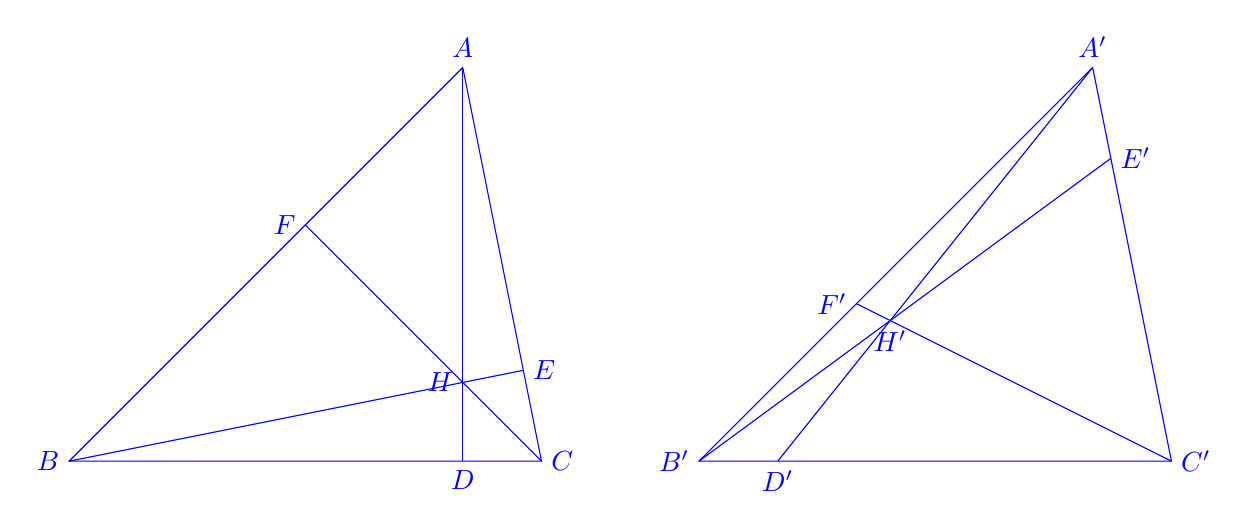
\begin{tikzpicture}
 \coordinate [label=above:\textcolor{blue}{$A$}] (A) at (5,5);
 \coordinate [label=left:\textcolor{blue}{$B$}] (B) at (0,0);
 \coordinate [label=right:\textcolor{blue}{$C$}] (C) at (6,0);
 \coordinate [label=below:\textcolor{blue}{$D$}] (D) at (5,0);
 \coordinate [label=left:\textcolor{blue}{$F$}](F) at (3,3);
 \coordinate [label=right:\textcolor{blue}{$E$}](E) at (150/26, 30/26);
 \coordinate [label=left:\textcolor{blue}{$H$}](H) at (5,1);
 
 \draw[blue] (A) -- (B) -- (C) -- (A);
 \draw[blue] (B) -- (E);
 \draw[blue] (C) -- (F);
 \draw[blue] (A) -- (D);
 
 \coordinate [label=above:\textcolor{blue}{$A'$}] (A') at (13,5);
 \coordinate [label=left:\textcolor{blue}{$B'$}] (B') at (8,0);
 \coordinate [label=right:\textcolor{blue}{$C'$}] (C') at (14,0);
 \coordinate [label=below:\textcolor{blue}{$D'$}] (D') at (9,0);
 \coordinate [label=left:\textcolor{blue}{$F'$}] (F') at (10,2);
 \coordinate [label=right:\textcolor{blue}{$E'$}] (E') at (172/13, 50/13);
 \coordinate [label=below:\textcolor{blue}{$H'$}] (H') at (73/7, 25/14);
 
  \draw[blue] (A') -- (B') -- (C') -- (A');
 \draw[blue] (B') -- (E');
 \draw[blue] (C') -- (F');
 \draw[blue] (A') -- (D');
\end{tikzpicture}
\ed

\bt{球面三角形余弦定理}{}
对于任给半径为$R$的球面三角形$\triangle ABC$, 其三边$a,b,c$和三角$\angle A, \angle B, \angle C$之间恒满足:
\begin{align*}
 \cos\frac{a}{R^2} & =\cos\frac{c}{R^2}\cos\frac{b}{R^2}+\sin\frac{b}{R^2}\sin\frac{c}{R^2}\cos\angle A,\\
 \cos\frac{b}{R^2} & =\cos\frac{a}{R^2}\cos\frac{c}{R^2}+\sin\frac{c}{R^2}\sin\frac{a}{R^2}\cos\angle B,\\
 \cos\frac{c}{R^2} & =\cos\frac{b}{R^2}\cos\frac{a}{R^2}+\sin\frac{a}{R^2}\sin\frac{b}{R^2}\cos\angle C.
\end{align*}
\et

\bt{球面三角形正弦定理}{}
条件同上, 有$\frac{\sin\angle A}{\sin\frac{a}{R^2}}=\frac{\sin\angle B}{\sin\frac{b}{R^2}}=\frac{\sin\angle C}{\sin\frac{c}{R^2}}$.
\et

\newpage

\section{inequality}
\bq{}{}
已知$0\le a_k\le 1$($k=1,2,\cdots, 2002$), 记$a_{2003}=a_1$, $a_{2004}=a_2$, 求$\sum_{k=1}^{2002}(a_k-a_{k+1}\cdot a_{k+2})$的最大值.
\eq
\ba
\bee
\sum_{k=1}^{2002}(a_k-a_{k+1}\cdot a_{k+2})=\sum_{k=1}^{2002}(a_k-a_{k}a_{k+1})=\sum_{k=1}^{2002}a_{k}(1-a_{k+1}).
\eee
Cauchy不等式, 上式右端不超过
\bee
\sqrt{\left(\sum_{k=1}^{2002}a_k^2\right)\left(\sum_{k=1}^{2002}(1-a_{k+1})^2\right)}
\le \frac{\sum a_k^2 + \sum (1-a_{k+1})^2}{2}
=\frac{\sum a_k^2+\sum(1-a_k)^2}{2}
=\frac{\sum(2a_k^2-2a_k+1)}{2}.
\eee
因为$2a_k^2-2a_k+1\le1$, 所以原式不超过$\frac12\sum1=1001$, 当$a_k=0$或$1$时取等号, 即当$a_1=a_3=a_5=\cdots=a_{2001}=1$且$a_2=a_4=\cdots=a_{2002}=0$时取等号.
\ea
\ba
由$0\le a_k\le 1$, 得$(1-a_k)(1-a_{k+1})=1-(a_{k}+a_{k+1})+a_{k}a_{k+1}\ge0$($k=1,2,\cdots, 2002$), 所以$1\ge a_{k}+a_{k+1}-a_{k}a_{k+1}\ge a_{k}+a_{k+1}-2a_{k}a_{k+1}$,
从而$2002\ge\sum_{k=1}^{2002}(a_k+a_{k+1}-2a_{k}a_{k+1})=2\sum(a_k-a_{k+1}a_{k+2})$, 即$\sum(a_k-a_{k+1}a_{k+2})\le1001$.
\ea

\bq{}{}
求函数$y=x+\sqrt{x(2-x)}$的最值及此时$x$的值.
\eq
\ba
显然$x\in[0,2]$, 所以可设$x=2\sin^2\theta$($\theta\in\mathbb{R}$), 运用$|a\sin\theta+b\cos\theta|\le\sqrt{a^2+b^2}$即可.
\ea

\bq{}{}
设$n$是给定的正整数, $n\ge13$, 对$n$个给定的实数$a_1, a_2, \cdots, a_n$, 记$|a_i-a_j|$($1\le i < j\le n$)有最小值$m$, 求在$\sum_{i=1}^{n}a_i^2=1$的条件下, 
$m$的最大值.
\eq
\ba
不妨设$a_1\le a_2\le \cdots\le a_n$, 于是$a_2-a_1\ge m, a_3-a_2\ge m, \cdots, a_n-a_{n-1}\ge m$, $a_j-a_i\ge(j-i)m$($1\le i< j \le n$).
\bee
\sum_{1\le i<j\le n}(a_i-a_j)^2\ge m^2\times\sum_{1\le i<j\le n}(j-i)^2
=m^2\sum_{k=1}^{n-1}k(2k+1)(k+1)=\frac{m^2}{12}\cdot n^2(n^2-1).
\eee
另一方面, $\sum_{i=1}^{n}a_i^2=1$可得
\bee
\sum_{1\le i<j\le n}(a_i-a_j)^2=n-\left(\sum_{i=1}^{n}a_i\right)^2\le n.
\eee
故$n\ge\frac{m^2}{12}n^2(n^2-1)$, 所以$m\le\sqrt{\frac{12}{n^2(n^2-1)}}$, 当且仅当$\sum_{i=1}^{n}a_i=0$,
且$a_1, a_2, \cdots, a_n$成等差数列时取等号.
\ea

\bq{}{}
若$x,y,z>0$且$x^2+y^2+z^2=1$, 则$S=\frac{(z+1)^2}{2xyz}$取最小值时, $x$的值是多少?
\eq
\ba
$\sqrt{\sqrt{2}-1}$.
\ea

\bl{}{}
设$T\ge0$, $x, y, z\ge0$, 则$T\ge\sum x$的充要条件为:
\begin{align}
 & (T^2-\sum x^2)^2-8\prod x\cdot T-4\sum y^2z^2\ge0\label{20170327001}\\
 & T^2\ge\sum x^2.\label{20170327002}
\end{align}
\el
\ba
若$T\ge\sum x$, 则\ref{20170327002}式明显成立, 且
\bee
(T+\sum x)(T^2-\sum x^2+2\sum yz)-8\prod x
\ge2\sum x\cdot 4\sum yz-8\prod x
\ge0.
\eee
根据
\be
(T^2-\sum x^2)^2-8\prod x\cdot T-4\sum y^2z^2
=(T-\sum x)\left[(T+\sum x)(T^2-\sum x^2+2\sum yz)-8\prod x\right]\label{20170327003}
\ee
知\ref{20170327001}式成立. 若\ref{20170327001}, \ref{20170327002}式成立, 则
\bee
(T+\sum x)(T^2-\sum x^2+2\sum yz)-8\prod x
\ge (\sqrt{\sum x^2}+\sum x)\cdot 2\sum yz-8\prod x
\ge (\sqrt{3}+3)(\prod x)^{\frac13}\cdot6(\prod x)^{\frac23}-8\prod x\ge0.
\eee
根据\ref{20170327003}式知$T\ge\sum x$.
\ea
由引理即得
\bt{}{20170328001}
设$T\ge0$, $x,y,z\ge0$, 记$f=(T^2-\sum x^2)^2-8\prod x\cdot T-4\sum y^2z^2$, 则
\begin{enumerate}[(i)]
 \item 若$f\ge0$, $\sum x^2\le T^2$, 则$\sum x\le T$;
 \item 若$f\le 0$, 则$\sum x\ge T$.
\end{enumerate}
\et

\bq{}{}
\bee
\sum\cos\frac{A}{2}\le2+\frac{s}{4R}+\frac{9\sqrt{3}-16}{4R}r.
\eee
\eq
\ba
设$m=\frac{s}{4R}$, $n=\frac{r}{2R}$. 则$\sum\cos^2\frac{A}{2}=2+n$, $\prod\cos\frac{A}{2}=\frac{m}{2}$. 进而
\bee
\sum\cos^2\frac{A}{2}\cos^2\frac{B}{2}=\frac14(4+4n+m^2+n^2).
\eee
令$T=2+\frac{m}{2}+\frac{9\sqrt{3}-16}{2}n$, $x=\cos\frac{A}{2}$, $y=\cos\frac{B}{2}$, $z=\cos\frac{C}{2}$,
用定理\ref{th:20170328001}中结论(i).
\ea

\bq{}{}
设实数$a,b,c,d$, 满足$a^2+b^2+c^2+d^2=5$, 求$(a-b)^2+(a-c)^2+(a-d)^2+(b-c)^2+(b-d)^2+(c-d)^2$的最大值.
\eq
\ba
设$f=(a-b)^2+(a-c)^2+(a-d)^2+(b-c)^2+(b-d)^2+(c-d)^2=15-2(ab+ac+ad+bc+bd+cd)+\lambda(a^2+b^2+c^2+d^2-5)$,
所以$f_a=-2(b+c+d)+2a\lambda$, $f_b=-2(a+c+d)+2b\lambda$, $f_c=-2(a+b+d)+2c\lambda$, $f_d=-2(a+c+d)+2b\lambda$,
$f_{\lambda}=a^2+b^2+c^2+d^2-5$, 令$f_a=f_b=f_c=f_d=f_{\lambda}=0$, 解得$\lambda=-1$或$a=b=c=d$.
当$\lambda=-1$时, $a+b+c+d=0$得$f=20$.
当$a=b=c=d$时, $f=0$, 所以$f_{\max}=20$.
\ea

\bq{}{}
如果$x>0$, $y>0$, $z>0$且$x^2+y^2+z^2=1$, 求$\frac{yz}{x}+\frac{xz}{y}+\frac{xy}{z}$的最小值.
\eq
\ba
设$\frac{yz}{x}=a$, $\frac{xz}{y}-b$, $\frac{xy}{z}=c$, 则
$ab+bc+ca=1$, 所以$a^2+b^2+c^2\ge ab+bc+ca=1$, 所以$(a+b+c)^2=a^2+b^2+c^2+2(ab+bc+ca)\ge3$,
另外令$f=a+b+c+\lambda(ab+bc+ca-1)$, 令
$f_a=1+(b+c)\lambda=0$, $f_b=1+(a+c)\lambda=0$, $f_c=1+(a+b)\lambda=0$, 所以
$a=b=c$时最小.
\ea

\bq{}{}
设$a_0, a_1, a_2, \cdots, a_n$满足$a_0=\frac12$, $a_{k+1}=a_k+\frac{1}{n}a_k^2$, $k=0,1,2,\cdots, n-1$,
其中$n$是一个给定的正整数, 试证: $1-\frac{1}{n}<a_n<1$.
\eq
\ba
$a_n>a_{n-1}>a_{n-2}>\cdots>a_2>a_1>a_0=\frac{1}{2}$,
\begin{align*}
 \frac{1}{a_k}-\frac{1}{a_{k+1}}=\frac{1}{n+a_k}<\frac{1}{n} \Longrightarrow\frac{1}{a_0}-\frac{1}{a_n}<1,\\
 \frac{1}{a_k}-\frac{1}{a_{k+1}}=\frac{1}{n+a_k}>\frac{1}{n+1} \Longrightarrow\frac{1}{a_0}-\frac{1}{a_n}>\frac{n}{n+1}.
\end{align*}
\ea

\bq{}{}
当$a>1$时, 若不等式$\frac{1}{n+1}+\frac{1}{n+2}+\cdots+\frac{1}{2n}>\frac{7}{12}\left[\log_{a+1}x-\log_{a}x+1\right]$对于不小于2的正整数$n$恒成立,
求$x$的取值范围.
\eq
\ba
$a_{n}=\frac{1}{n+1}+\frac{1}{n+2}+\cdots+\frac{1}{2n}$递增, $x$的取值范围为$(1, +\infty)$.
\ea

\bq{}{}
实数集$\{a_0, a_1, a_2, \cdots, a_n\}$, 满足以下条件: 
\begin{enumerate}[(1)]
 \item $a_1=a_n=0$.
 \item 对$1\le k\le n-1$, 有$a_k=c+\sum_{i=k}^{n-1}a_{i-k}(a_i+a_{i+1})$.
\end{enumerate}
证明: $c\le\frac{1}{4n}$.
\eq
\ba
定义$S_k=\sum_{i=0}^ka_i$($k=0,1,2,\cdots, n$), 则
\begin{align*}
 S_n
 & =\sum_{k=0}^{n}a_k
 =\sum_{k=0}^{n-1}a_{k-1}
 =nc+\sum_{k=0}^{n-1}\sum_{i=k}^{n-1}a_{i-k}(a_i+a_{i+1})\\
 & =nc+\sum_{i=0}^{n-1}(a_i+a_{i+1})\cdot\sum_{k=0}^{i}a_{i-k}\\
 & =nc+\sum_{i=0}^{n-1}(a_i+a_{i+1})\sum_{t=0}^{i}a_t, (t=i-k)\\
 & =nc+\sum_{i=0}^{n-1}(a_i+a_{i+1})\cdot S_i\\
 & =nc+\left[S_1S_0+(S_2-S_0)S_1+(S_3-S_1)S_2+\cdots+(S_n-S_{n-2})S_{n-1}\right]
\end{align*}
即$S_n^2-S_n+nc=0$, $\Delta\ge0\Longrightarrow c\le\frac{1}{4n}$.
\ea

\bq{}{}
若关于$x$的不等式$\log_{\frac{1}{a}}(\sqrt{x^2+ax+5}+1)\cdot\log_{5}(x^2+ax+6)+\frac{1}{\log_{3}a}\ge0$,
求$a$的取值范围.
\eq
\ba
令$u=x^2+ax+5$, $\frac{\log_3(\sqrt{u}+1)}{-\log_3a}\cdot\log_5(u+1)+\frac{1}{\log_3a}\ge0$.
因为$f(4)=1$, 所以$a=2$.
\ea

\bq{}{}
设$a_1, a_2, \cdots, a_{2002}>0$且$\sum\frac{1}{2+a_i}=\frac12$, 求$\prod a_i$的最小值.
\eq
\ba
令$x_i=\frac{2}{2+a_i}$, 则$\sum x_i=1$, 则$a_i=2\cdot\frac{1-x_i}{x_i}$, 
因为
\begin{align*}
 \prod a_i
 & =2^{2002}\prod\frac{1-x_i}{x_i}\\
 & =2^{2002}\cdot\frac{1}{x_1x_2\cdots x_{2002}}\prod(x_1+x_2+\cdots+x_{i-1}+x_{i+1}+\cdots+x_{2002})\\
 & \ge2^{2002}\cdot\frac{1}{x_ix_2\cdots x_{2002}}\cdot2001^{2002}\cdot\prod\sqrt[2001]{x_1x_2\cdots x_{i-1}x_{i+1}\cdots x_{2002}}\\
 &=4002^{2002}.
\end{align*}
\ea

\bq{}{}
求最小的正数$\lambda$, 使得对任意正整数$n$, $a_i$和$b_i$, $b_i\in[1,2]$($i=1,2,\cdots, n$), 且$\sum_{i=1}^{n}a_{i}^2=\sum b_i^2$, 
都有$\sum\frac{a_i^3}{b_i}\le\lambda\cdot\sum a_i^2$.
\eq
\ba
对任意$c_i, b_i\in[1,2]$, 有$\frac{1}{2}\le\frac{c_i}{b_i}\le 2$, 即$\frac{1}{2}b_i\le c_i\le2b_i$,
从而$\left(\frac{1}{2}b_i-c_i\right)(2b_i-c_i)\le0$, 即$c_i^2+b_i^2\le\frac{5}{2}c_ib_i$,
两边对$i$从1到$n$求和, 得$\sum c_i^2+\sum b_i^2\le\frac{5}{2}\sum c_ib_i$,
设$a_i, b_i\in\left[1, \frac{2}{3}\right]$, 因$a_i^2=\frac{a_i^{\frac{3}{2}}}{b_i^{\frac{1}{2}}}\cdot a_i^{\frac{1}{2}}\cdot b_i^{\frac{1}{2}}$.
又
\bee
\frac{1}{2}\le\frac{\frac{a_i^{\frac{3}{2}}}{b_{i}^{\frac{1}{2}}}}{a_i^{\frac{1}{2}}\cdot b_i^{\frac{1}{2}}}\le 2.
\eee
故有$\frac{5}{2}\sum a_i^2\ge\sum\frac{a_i^3}{b_i}+\sum a_ib_i\ge\sum\frac{a_i^3}{b_i}+\frac{2}{5}(\sum a_i^2+\sum b_i^2)=\sum\frac{a_i^3}{b_i}+\frac{4}{5}\sum a_i^2$,
即$\sum\frac{a_i^3}{b_i}\le\frac{17}{10}\sum a_i^2$, 当$n=2$, $a_1=1$, $a_2=2$, $b_1=2$, $b_2=1$时取等号.
\ea

\bq{}{}
已知: $x,y,z\in\mathbb{R}^*$, 有$xyz=1$且满足$x(1+z)>1$, $y(1+x)>1$, $z(1+y)>1$, 
求证: $2(x+y+z)\ge\frac{1}{x}+\frac{1}{y}+\frac{1}{z}+3$.
\eq
\ba
令$x=\frac{a}{b}$, $y=\frac{b}{c}$, $z=\frac{c}{a}$, 则$a+c>b$, $a+b>c$, $b+c>a$, 要证$2(x+y+z)\ge\frac1x+\frac1y+\frac1z+3$, 只需证
\bee
2\left(\frac{a}{b}+\frac{b}{c}+\frac{c}{a}\right)\ge\frac{b}{a}+\frac{c}{b}+\frac{a}{c}+3\Longleftrightarrow
  2(a^2c+b^2a+c^2b)\ge b^2c+c^2a+a^2b+3abc.
\eee
因为
\bee
(a+b-c)(b-c)^2\ge0, \quad (b+c-a)(c-a)^2\ge0, \quad (c+a-b)(a-b)^2\ge0
\eee
展开相加, 即得.
\ea

\bq{}{}
已知正整数$n\ge 2$, 若对同时满足条件:
\begin{enumerate}[(1)]
 \item $a_1a_2\cdots a_n=b_1 b_2\cdots b_n$;
 \item $\sum_{1\le i<j\le n}|a_i-a_j|\le \sum_{1\le i<j\le n}|b_i-b_j|$的任意正数$a_1,\cdots, a_n$与$b_1,\cdots, b_n$,
 总有$\sum_{i=1}^{n}a_i\le\lambda\sum_{i=1}^{n}b_i$. 试求正数$\lambda$的最小值.
\end{enumerate}
\eq
\ba
一方面, 取$(a_1,\cdots, a_n)=(1,1,\cdots,(1+x)x^{n-1})$, $(b_1,\cdots,b_n)=(1+x,x,x,\cdots, x)$, 满足(1)与(2), 
此时$\lambda\ge\frac{\sum a_i}{\sum b_i}=\frac{n-1+x^{n-1}+x^n}{1+nx}$, 令$x\to0$, 则$\lambda\ge n-1$.

以下证明$\lambda=n-1$时, 不等式成立.

不妨设$a_1\ge a_2\ge\cdots\ge a_n$, $b_1\ge b_2\ge \cdots\ge b_n$, $n=2$时, 显然成立.

设$n\ge3$,

(1) 若$a_1\le\frac{n-1}{n}b_1$, 则$\sum a_i\le na_1\le(n-1)b_1\le(n-1)\sum b_i$.

(2) 若$a_1>\frac{n-1}{n}b_1$, 则
\begin{align*}
 2(b_2+\cdots+b_n) & \ge 2(n-1)\cdot(b_2\cdots b_n)^{\frac{1}{n-1}}=2(n-1)\left(\frac{a_1}{b_1}a_2\cdots a_n\right)^{\frac{1}{n-1}}\\
  & \ge 2(n-1)\left(\frac{a_1}{b_1}\right)^{\frac{1}{n-1}}\cdot a_n>2(n-1)\cdot\left(\frac{n-1}{n}\right)^{\frac{1}{n-1}}\cdot a_n\\
  & \ge na_n.
\end{align*}
所以
\begin{align*}
 (n-1)\sum b_i &= (n-1)b_1+(n-3)\sum_{i=2}^{n}b_i+2\sum_{i=2}^{n}b_i\\
  &\ge(n-1)b_1+(n-3)\sum_{i=2}^{n}b_i+na_n\ge[(n-1)b_1+(n-3)b_2+\cdots-(n-1)b_n]+na_n\\
  &=\sum_{1\le i<j\le n}|b_i-b_j|+na_n\ge\sum_{1\le i<j\le n}|a_i-a_j|+na_n\\
  &=[(n-1)a_1+(n-3)a_2+\cdots-(n-1)a_n]+na_n\\
  &\ge(n-1)a_1+a_n\ge a_1+a_2+\cdots+a_{n-1}+a_n.
\end{align*}
\ea

\bq{1998年上海市高中数学竞赛}{}
设非零多项式$f(x)=a_nx^n+a_{n-1}x^{n-1}+\cdots+a_0$, $g(x)=c_{n+1}x^{n+1}+c_nx^n+\cdots+c_0$, 满足$g(x)=(x+r)f(x)$, 其中$r$为一实数,
设$a=\max(|a_{n}|, |a_{n-1}|,\cdots,|a_0|)$, $c=\max(|c_{n+1}|,|c_{n}|,\cdots,|c_0|)$, 求证: $\frac{a}{c}\le n+1$.
\eq
\ba
设$|r|\le1$, 由$\sum_{i=0}^{n+1}c_ix^i=(x+r)\sum_{i=0}^{n}a_ix^i=a_nx^{n+1}+\sum_{i=1}^{n}(ra_i+a_{i-1})x^i+ra_0$. 
故
\bee
\begin{dcases}
 c_{n+1}=a_n\\
 c_{n}=ra_n+a_{n-1}\\
 \cdots\\
 c_{1}=ra_1+a_0\\
 c_0=ra_0
\end{dcases}
\Longrightarrow
\begin{dcases}
 a_{n}=c_{n+1}\\
 a_{n-1}=-rc_{n+1}+c_n\\
 a_{n-2}=(-r)^2c_{n+1}+(-r)c_n+c_{n-1}\\
 \cdots\\
 a_0=(-r)^nc_{n+1}+(-r)^{n-1}c_n+\cdots+c_1,
\end{dcases}
\eee
故$|a|=|a_i|=|(-r)^{n-i}c_{n+1}+\cdots+c_{i+1}|\le|c_{n+1}|+\cdots+|c_{i+1}|\le(n-i+1)c\le(n+1)c$.

如果$|r|>1$, 令$x=\frac{1}{x}$, 代入$g(x)=(x+r)f(x)$, 则转化为上述情形, 仍有$a\le(n+1)c$.

另外
\bee
  |a|=|a_i|\le|r|^{n-i}|c_{n+1}|+\cdots+|c_{i+1}|\le(|r^n|+|r^{n-1}|+\cdots+1)c\le\frac{|r|^{n+1}-1}{|r|-1}c
\eee
而
\bee
\frac{|r|^{n+1}-1}{|r|-1}\le n+1
\Longleftrightarrow |r|^{n+1}\ge n|r|-n+|r|
\Longleftrightarrow |r|^n+\frac{n}{|r|}\ge n+1
\Longleftrightarrow |r|^n+\frac{1}{|r|}+\cdots+\frac{1}{|r|}\ge n+1
\eee

($|r|=0$时, 命题显然成立).
\ea

\bq{}{}
若$a,b,c\in\mathbb{R}$, 且$5a^4+4b^4+6c^4=90$, 求$5a^3+2b^3+3c^3$的最大值.
\eq
\ba
只需考虑$a,b,c\in\mathbb{R}^*$. 因$a^3=\frac12(a\cdot a\cdot a\cdot2)\le\frac{1}{8}(a^4+a^4+a^4+2^4)=\frac38a^4+2$,
同理$b^3\le\frac34b^4+\frac14$, $c^3\le\frac34c^4+\frac14$, 所以所求最大值为$45$.
\ea

\bq{}{}
若$x,y,z$为实数, $0<x<y<z<\frac{\pi}{2}$, 证明: $\frac{\pi}{2}+2\sin x\cos y+2\sin y\cos z>\sin 2x+\sin 2y+\sin 2z$.
\eq
\ba
原不等式等价于证明$\frac{\pi}{4}>\sin x(\cos x-\cos y)+\sin y(\cos y-\cos z)+\sin z\cos z$. 如图所示
\begin{center}
 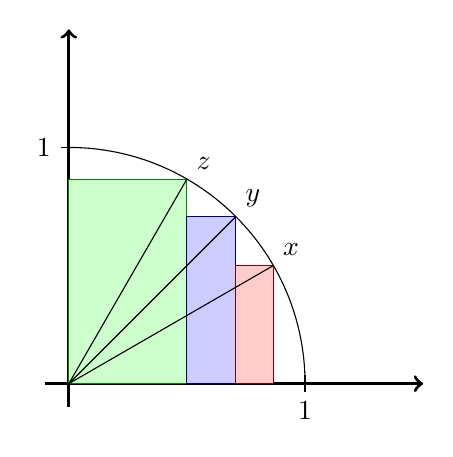
\begin{tikzpicture}[scale=3]
  \draw[->,very thick] (-.1,0) -- (1.5,0) coordinate (x axis);
  \draw[->,very thick] (0,-0.1) -- (0,1.5) coordinate (y axis);
  \draw (1,0) arc [start angle=0,end angle=90,x radius=1cm,y radius=1cm];
  let x=30;
  let y=45;
  let z=60;
  \filldraw[fill=green!20, draw=green!50!black] (0,0) -- (0.5,0) -- (0.5,0.866) -- (0,0.866) -- cycle;
  \filldraw[fill=blue!20, draw=blue!50!black] (0.5,0) -- (0.707,0) -- (0.707,0.707) -- (0.5,0.707) -- cycle;
  \filldraw[fill=red!20, draw=red!50!black] (0.707,0) -- (0.866,0) -- (0.866,0.5) -- (0.707,0.5) -- cycle;
  \draw (0,0) -- (0.866,0.5) node [anchor=south west] {$x$};
  \draw (0,0) -- (0.707,0.707) node [anchor=south west] {$y$};
  \draw (0,0) -- (0.5,0.866) node [anchor=south west] {$z$};
  \draw (1,1pt) -- (1,-1pt) node [anchor=north] {$1$};
  \draw (1pt,1) -- (-1pt,1) node [anchor=east] {$1$};
  \end{tikzpicture}
\end{center}
\ea

\bq{1987年第21届全苏MO}{}
正数$a,b,c,A,B,C$满足条件$a+A=b+B=c+C=k$, 求证: $aB+bC+cA<k^2$.
\eq
\ba
主试委员会给出的解答是$k^3=(a+A)(b+B)(c+C)$, 利用放缩的技巧给出证明, 北京四中的袁峰同学给出了如下构造性证明.

如图: $S_{\triangle LRM}+S_{\triangle PNM}+S_{\triangle QLN}<S_{\triangle PQR}$, 化简即得.
\begin{center}
 \begin{tikzpicture}[scale=3]
  \coordinate [label=left:$Q$] (Q) at (0,0);
  \coordinate [label=above:$P$] (P) at (0.5,0.866);
  \coordinate [label=right:$R$] (R) at (1,0);
  \draw (P) -- (Q) -- (R) -- cycle;
  \coordinate [label=below:$L$] (L) at ($ (R) !0.7! (Q) $);
  \coordinate [label=right:$M$] (M) at ($ (P) !0.4! (R)$);
  \coordinate [label=left:$N$] (N) at ($ (P) !0.5! (Q)$);
  \draw (L) -- (M) -- (N) -- cycle;
  \node (A) [label=below:$A$] at ($ (Q) !0.5! (L) $) {};
  \node (a) [label=below:$a$] at ($ (R) !0.5! (L) $) {};
  \node (B) [label=right:$B$] at ($ (M) !0.5! (R) $) {};
  \node (b) [label=right:$b$] at ($ (P) !0.5! (M) $) {};
  \node (C) [label=left:$C$] at ($ (P) !0.5! (N) $) {};
  \node (c) [label=left:$c$] at ($ (N) !0.5! (Q) $) {};
  
  \foreach \point in {P,Q,R,L,M,N}
    \fill [blue,opacity=.75] (\point) circle (1pt);
 \end{tikzpicture}

\end{center}

\ea
\ba
如图:
\begin{center}
 \begin{tikzpicture}[scale=3]
  \coordinate[label=225:$P$] (P) at (0,0);
  \coordinate[label=315:$Q$] (Q) at (1,0);
  \coordinate[label=45:$R$] (R) at (1,1);
  \coordinate[label=135:$S$] (S) at (0,1);
  
  \draw (P) -- (Q) -- (R) -- (S) -- cycle;
  \filldraw[fill=yellow!80!black,opacity=0.5] (P) rectangle (0.6,0.4);
  \filldraw[fill=red!80!black,opacity=0.5] (0.6,0) rectangle (1,0.7);
  \filldraw[fill=blue!80!black,opacity=0.5] (1,0.7) rectangle (0.3,1);
  
  \node [label=below:$B$] at ( $ (P) !0.5! (0.6,0) $) {};
  \node [label=below:$b$] at ( $ (Q) !0.5! (0.6,0) $) {};
  \node [label=right:$C$] at ( $ (Q) !0.5! (1,0.7) $) {};
  \node [label=right:$c$] at ( $ (R) !0.5! (1,0.7) $) {};
  \node [label=above:$A$] at ( $ (R) !0.5! (0.3,1) $) {};
  \node [label=left:$a$] at ( $ (P) !0.5! (0,0.4) $) {};
  
  \foreach \point in {P,Q,R,S}
    \fill [blue,opacity=.75] (\point) circle (1pt);
 \end{tikzpicture}

\end{center}

\ea

\bq{第31届IMO预选题}{}
设集合$\{a_1,a_2,\cdots,a_n\}=\{1,2,\cdots,n\}$, 求证:
\bee
\frac12+\frac23+\cdots+\frac{n-1}{n}\le\frac{a_1}{a_2}+\frac{a_2}{a_3}+\cdots+\frac{a_{n-1}}{a_n}.
\eee
\eq
\ba
设$b_1,b_2,\cdots,b_{n-1}$是$a_1,a_2,\cdots,a_{n-1}$的一个排列, 且$b_1<b_2<\cdots<b_{n-1}$, 
$c_1,c_2,\cdots,c_{n-1}$是$a_2,a_3,\cdots,a_{n}$的一个排列, 且$c_1<c_2<\cdots<c_{n-1}$, 则
\bee
\frac1{c_1}>\frac1{c_2}>\cdots>\frac1{c_{n-1}}.
\eee
且$b_1\ge1$, $b_2\ge2$, $\cdots,b_{n-1}\ge n-1$, $c_1\le 2,c_2\le3,\cdots,c_{n-1}\le n$,
由排序不等式得:
\bee
\frac{a_1}{a_2}+\frac{a_2}{a_3}+\cdots+\frac{a_{n-1}}{a_n}
  \ge \frac{b_1}{c_1}+\frac{b_2}{c_2}+\cdots+\frac{b_{n-1}}{c_{n-1}}
  \ge \frac12+\frac23+\cdots+\frac{n-1}{n}.
\eee
这是南斯拉夫提给第31届IMO的一道试题, 原证法是利用加强命题的手法, 用数学归纳法给出证明.
一则加强命题很难想到, 二则归纳法证明要对足标进行讨论, 比较麻烦. 在当年国家集训队里姚建钢同学(第35届IMO金牌得主)的证法,
更是干脆, 漂亮, 出人意料.
\ea
\ba
易证
\bee
\prod_{k=1}^{n-1}(a_k+1)\ge\prod_{k=1}^na_k,
\eee
故
\begin{align*}
 \sum_{k=1}^{n-1}\frac{a_k}{a_{k+1}}+\paren{\sum_{k=1}^n\frac1k}
  &=\frac{1}{a_1}+\sum_{k=1}^{n-1}\frac{a_k+1}{a_{k+1}}\\
  &\ge n \sqrt[n]{\frac{\prod_{k=1}^{n-1}(a_k+1)}{\prod_{k=1}^na_k}}\ge n\\
  &=\sum_{k=1}^{n}\frac{1}{k}+\sum_{k=1}^{n-1}\frac{k}{k+1}
\end{align*}

\ea

\bq{第24届IMO}{}
设$a,b,c$分别为一个三角形的三边之长, 求证:
\bee
a^2b(a-b)+b^2c(b-c)+c^2a(c-a)\ge0.
\eee
并指出等号成立的条件.
\eq
\ba
原联邦德国选手伯恩哈德$\cdot$里普只用了一个等式:
\bee
a^2b(a-b)+b^2c(b-c)+c^2a(c-a)
  = a(b-c)^2(b+c-a)+b(a-b)(a-c)(a+b-c)
\eee
由轮换对称性, 不妨设$a\ge b, c$, 即得欲证不等式成立, 而且显然等号成立的充要条件是$a=b=c$.

里普的证法新颖, 巧妙, 简洁, 与主试委员会提供的参考答案不同, 他因此获得了该届的特别奖.
\ea

\bq{1980年芬兰, 英国, 匈牙利, 瑞典四国联赛}{}
设数列$a_0,a_1,\cdots,a_n$满足$a_0=\frac12$及$a_{k+1}=a_k+\frac1na_k^2$($k=0,1,2,\cdots,n-1$),
其中$n$是一个给定的正整数, 试证:
\bee
1-\frac1n<a_n<1.
\eee
\eq
\ba
该题是该次竞赛得分率最低的一道试题, 主试委员会所给出的解法也相当繁琐, 前后共用了四次归纳法, 译成中文后有4000多字,
中国科技大学白志东先生对此题采用了大胆的处理方法, 加强命题, 出奇制胜给出一个简洁的证明.

由于$a_1=a_0+\frac1na_0^2=\frac12+\frac1{4n}=\frac{2n+1}{4n}$, 所以
\bee
\frac{n+1}{2n+1}<a_1<\frac{n}{2n-1}.
\eee
我们来用归纳法证: 对于一切$1\le k\le n$, 都有
\be\label{20180704001}
\frac{n+1}{2n-k+2}<a_k<\frac{n}{2n-k}.
\ee
假设(\ref{20180704001})对于$k<n$成立, 则
\bee
a_{k+1}=a_k\paren{1+\frac1na_k}
  <\frac{n}{2n-k}\paren{1+\frac1{2n-k}}
  =\frac{n(2n-k+1)}{(2n-k)^2}
  <\frac{n}{2n-(k+1)}.
\eee
所以
\begin{align*}
 a_{k+1} & = a_k+\frac1na_k^2>\frac{n+1}{2n-k+2}+\frac{(n+1)^2}{n(2n-k+2)^2}\\
  &>\frac{n+1}{2n-(k+1)+2}
\end{align*}
于是(\ref{20180704001})式对于一切$1\le k\le n$均成立, 特别在$k=n$时,
\bee
1-\frac1n<\frac{n+1}{n+2}<a_n<\frac{n}{n}=1.
\eee

{\bf{说明}} 这里所证的不等式(\ref{20180704001})式比题目所要证明的不等式强, 却收到了事半功倍之效,
下面给出一种直接了当的证明.
\ea
\ba
由已知, 
\bee
\frac1{a_{k-1}}-\frac1{a_k}=\frac1{n+a_{k-1}},
\eee
从而$a_n>a_{n-1}>\cdots>a_1>a_0=\frac12$. 所以
\bee
\frac1{a_{k-1}}-\frac1{a_k}<\frac1n,\quad k=1,2,\cdots,n.
\eee
累加得$\frac1{a_0}-\frac1{a_n}>\frac{n}{n+1}$, 所以$\frac{1}{a_n}<2-\frac{n}{n+1}=\frac{n+2}{n+1}$.
\ea

\bq{}{}
已知函数$f(x)$的定义域为$\RR$, 对于任意实数$m,n$均有$f(m+n)=f(m)+f(n)-1$, 且$f\paren{\frac12}=2$, 
当$x>-\frac12$时, 恒有$f(x)>0$, 求证: $f(x)$单调递增.
\eq
\ba
证明: 令$x_1>x_2$, 所以
\bee
f(x_1)-f(x_2)=f(x_1-x_2)-1
  =f\paren{\paren{x_1-x_2-\frac12}+\frac12}-1
  =f\paren{x_1-x_2-\frac12}+f\paren{\frac12}-1-1
  =f\paren{x_1-x_2-\frac12}
\eee
因为$x_1-x_2-\frac12>-\frac12$, 所以$f\paren{x_1-x_2-\frac12}>0$, 
所以$f(x_1)>f(x_2)$, 得证.
\ea

\bq{}{}
已知: 正数$x,y,z$均小于$1$且$x+y+z=2$, $w=xy+yz+zx$, 求$w$的取值范围.
\eq
\ba
易得$w\le\frac43$, 令$x(1-x)=a^2$, $y(1-y)=b^2$, $z(1-z)=c^2$, 因为
\bee
w=xy+z(2-z)=xz+y(2-y)=yz+x(2-x)
\eee
所以
\bee
3w=w+2\times2-x^2-y^2-z^2=w+4+a^2+b^2+c^2-2
\eee
所以$2w=2+a^2+b^2+c^2\ge2$, 即$w\ge1$.
仅当$a,b,c=0$时取$w=1$, 但$a,b,c\ne0$, 所以$w>1$.
\ea

\bq{}{}
已知$\frac{a^2+b^2}{4}+c^2=1$, 求$a+b+c$的最大值.
\eq
\ba
\begin{align*}
 (a+b+c)^2 = & a^2+b^2+c^2+2bc+2ab+2ac\\
  \le & a^2+b^2+c^2+(a^2+b^2)+\paren{\frac{b^2}{4}+4c^2}+\paren{\frac{a^2}{4}+4c^2}\\
  = & 9\paren{\frac{a^2+b^2}{4}}=9.
\end{align*}
\ea

\bq{}{}
已知$a,b>0$, $a+b=1$, 证明: $\frac32<\frac1{a^2+1}+\frac1{b^2+1}\le\frac85$.
\eq
\ba
原式等价于证明:
\begin{align*}
 15(a^2+1)(b^2+1)<10(a^2+b^2+2)\le16(a^2+1)(b^2+1)
  & \Longleftrightarrow 15a^2b^2+5a^2+5b^2-5<0\le16a^2b^2+6a^2+6b^2-4\\
  & \Longleftrightarrow 3a^2b^2+a^2+b^2-1<0\le8a^2b^2+3a^2+3b^2-2.
\end{align*}
因$a+b=1$, 所以$a^2+b^2-1=-2ab$. 所以上式等价于
\bee
3a^2b^2-2ab<0\le8a^2b^2-6ab+1.
\eee
又由$a^2+b^2+2ab=1\ge4ab$, 所以$0<ab\le\frac14$, 所以上式成立.
\ea
\ba
令$a=\sin^2\theta, b=\cos^2\theta$, $\paren{0<\theta<\frac{\pi}{2}}$, 所以
\begin{align*}
\frac1{a^2+1}+\frac1{b^2+1}
  &=\frac1{1+\sin^4\theta}+\frac1{1+\cos^4\theta}\\
  &=\frac4{5-2\cos2\theta+\cos^22\theta}+\frac4{5+2\cos2\theta+\cos^22\theta}\\
  &=\frac{16(11+\cos4\theta)}{(11+\cos4\theta)^2-8(11+\cos4\theta)+80}\\
  &=\frac{16y}{y^2-8y+80}=\frac{16}{y+\frac{80}{y}-8}
\end{align*}
因$0<\theta<\frac{\pi}{2}$, 所以$0<4\theta<2\pi$. 所以$10<y\le12$, 并有$\frac32<\frac{16}{y+\frac{80}{y}-8}\le\frac85$.
\ea

\bq{}{}
已知数列$\{a_n\}$, $\{b_n\}$, $\{c_n\}$满足: $b_n=a_n-a_{n+2}$, $c_n=a_n+2a_{n+1}+3a_{n+2}$, ($n=1,2,3,\cdots$),
若$\{c_n\}$为等差数列且$b_n\le b_{n+1}$, 证明: $b_n=b_{n+1}$.
\eq
\ba
由于$a_n-a_{n+2}=b_{n}\le b_{n+1}\le b_{n+2}=a_{n+2}-a_{n+4}$, 所以$2a_{n+2}\ge a_n+a_{n+4}$.
因为$2c_{n+1}=c_n+c_{n+2}$, 所以$4a_{n+3}=a_{n}+3a_{n+4}\le 2a_{n+2}+2a_{n+4}$, 
所以$2a_{n+3}\le a_{n+2}+a_{n+4}$. 所以$a_{n+3}-a_{n+2}\le a_{n+4}-a_{n+3}\le a_{n+5}-a_{n+4}$, 
所以$a_{n+3}-a_{n+5}\le a_{n+2}-a_{n+4}$, 所以$b_{n+3}\le b_{n+2}\le b_{n+3}$,
所以$b_{n+3}=b_{n+2}$, ($n\ge1$). 所以$b_3=b_4=b_5=\cdots=-2d=a_3-a_5=a_4-a_6=a_5-a_7$, 
所以
\begin{align*}
 4a_5-3a_6=a_2\le a_3-a_5+a_4
 &\Longrightarrow 5a_5\le a_3+a_4+3a_6\\
 &\Longrightarrow 5(a_3+2d)\le a_3+a_4+3(a_4+2d)\\
 &\Longrightarrow 2a_3\le2a_4-2d=2a_4+a_3-a_5\\
 &\Longrightarrow a_3+a_5\le 2a_4.
\end{align*}
因$a_3+a_5\ge2a_4$, 所以$a_2=a_3-a_5+a_4$, 同理$a_1=a_2-a_4+a_3$,
即$b_1=b_2=b_3=\cdots$.

两个正数$a,b$的和一定时, 它们的积
\be
ab=\frac14\paren{(a+b)^2-(a-b)^2}
\ee
随着差$\abs{a-b}$的增大而减小;
其平方和
\be
a^2+b^2=\frac12\paren{(a+b)^2+(a-b)^2}
\ee
随着差$\abs{a-b}$的增大而增大.
\ea

\bq{}{}
已知$\triangle ABC$的三边, $a, b,c$成等比数列, 则$\sin B+\cos B$的取值范围为\underline{$\qquad$}.
\eq
\ba
命题等价于$a+b>c$, $a+c>b$, $b+c>a$, $b^2=ac$,
\bee
b^2=ac=a^2+c^2-2ac\cos B\ge2ac-2ac\cos B,
\eee
所以$\cos B\ge\frac12$, $0<B\le60^{\circ}$, 由$\frac12\le\cos B<1$及$0<\sin B\le\frac{\sqrt{3}}{2}$,
所以
\be\label{20180705001}
\frac12<\cos B+\sin B<\frac{\sqrt{3}}{2}+1,
\ee
另一方面, $\sin B+\cos B=\sqrt{2}\sin(B+45^{\circ})$, 而$45^{\circ}<B+45^{\circ}<105^{\circ}$,
故
\be\label{20180705002}
1<\sin B+\cos B\le \sqrt{2}.
\ee
综合(\ref{20180705001}), (\ref{20180705002})有$1<\sin B+\cos B\le\sqrt{2}$.
\ea

\bq{}{}
设$a,b,c$是直角$\triangle ABC$的三边长, $c$为斜边, 求使不等式
\bee
a^2(b+c)+b^2(c+a)+c^2(a+b)\ge kabc
\eee
恒成立的$k$的最大值.
\eq
\ba
$a>0, b>0, c>0$, $c^2=a^2+b^2$, 所以
\begin{align*}
 LHS&=(a^2+b^2)c+a\paren{b^2+\frac{c^2}{2}}+b\paren{\frac{c^2}{2}+a^2}+\frac{c}{2}\cdot c(a+b)\\
  &\ge 2abc+\sqrt{2}abc+\sqrt{2}abc+\frac{c}{2}\sqrt{a^2+b^2}\cdot2\sqrt{ab}\\
  &\ge (2+2\sqrt{2})abc+c\cdot\sqrt{2ab}\cdot\sqrt{ab}=(2+3\sqrt{2})abc,
\end{align*}
仅当$a=b$时上式取等号.
\bee
(a+b+c)\paren{\frac1a+\frac1b+\frac1c}\ge5+3\sqrt{2}.
\eee
\ea

\bq{}{}
设$x_1$是方程$\sqrt{3}\sin x-3\cos x=2a-1$的最大负根, $x_2$是方程$2\cos^2 x-2\sin^2x=a$的最小正根,
求使不等式$\abs{x_1}\le x_2$成立的实数$a$的取值范围.
\eq
\ba
方程$\sqrt{3}\sin x-3\cos x=2a-1$等价于$\sin\paren{x-\frac{\pi}{3}}=\frac{2a-1}{2\sqrt{3}}$, 
从而得到$-1\le \frac{2a-1}{2\sqrt{3}}\le 1$. 解得$\frac12-\sqrt{3}\le a\le \frac12+\sqrt{3}$, 而且
\bee
x_1=
\begin{cases}
	\frac{\pi}{3}+\arcsin\frac{2a-1}{2\sqrt{3}}, & \paren{\frac12-\sqrt{3}\le a<-1}\\
	-\frac{2\pi}{3}-\arcsin\frac{2a-1}{2\sqrt{3}}, & \paren{-1\le a\le\frac12+\sqrt{3}}
\end{cases}
\eee
其图像如图, 位于$a$轴下方, 方程$2\cos^2x-2\sin^2x=a$等价于$\cos 2x=\frac{a}{2}$,
其中$-1\le\frac{a}{2}\le 1$, 所以$-2\le a\le 2$, 解得
\bee
x_2=
\begin{cases}
	\frac12\arccos\frac{a}{2}, & (-2<a\le 2)\\
	\pi, & (a=2).
\end{cases}
\eee
其图像如图, 它位于$a$轴上方, 比较两个函数的图像, 不难看出$|x_1|\le x_2$的充要条件是$\frac12-\sqrt{3}\le a\le -1$或$a=2$.
\begin{center}
 \begin{tikzpicture}
  \begin{axis}[
    axis equal,
    axis lines=middle,
    axis line style={->},
    xlabel={$a$},
    ylabel={$x$},
    ]
   \addplot[blue,thick] gnuplot [domain=-1.232:-1,samples=120] {pi/3+asin((2*x-1)/(2*sqrt(3)))};
   \addplot[blue,thick] gnuplot [domain=-1:2.232,samples=120] {-2*pi/3-asin((2*x-1)/(2*sqrt(3)))};
   \addplot[blue,thick] gnuplot [domain=-2:2,unbounded coords=jump,samples=120] {0.5*acos(x/2)};
   \addplot[
    scatter,
    only marks,
    nodes near coords,
    point meta=explicit symbolic,
    scatter/classes={
      o={mark=*,fill=white},
      c={mark=*,blue}},
   ] table[meta=label] {
      x		y	label
      2	3.14	c
      2	0	o
      -2	1.57	c
      -1	0	o
      -1.232	-0.52	c
      -1	-1.04	c
      2.232	-3.66	c
    };
    \addplot [color=blue, thick, dashed] coordinates {(2,0) (2,3.14) (0,3.14)};
    \addplot [color=blue, thick, dashed] coordinates {(-2,0) (-2,1.57) (0,1.57)};
    \addplot [color=blue, thick, dashed] coordinates {(-1.232,0) (-1.232,-0.52) (0,-0.52)};
    \addplot [color=blue, thick, dashed] coordinates {(-1,0) (-1,-1.04) (0,-1.04)};
    \addplot [color=blue, thick, dashed] coordinates {(2.232,0) (2.232,-3.66) (0,-3.66)};
    \addplot+[only marks,nodes near coords,blue,point meta=explicit symbolic] coordinates {
      (-2,1.57) [$(-2,\frac{\pi}{2})$]
      (2,3.14) [$(2,\pi)$]
    };
  \end{axis}
 \end{tikzpicture}
\end{center}
\ea

\bq{}{}
函数$y=\sqrt{8x-x^2}-\sqrt{14x-x^2-48}$的最大值为\underline{$2\sqrt{3}$}, 最小值为\underline{0}.
\eq
\ba
$x$的定义域为$6\le x \le 8$, 而
\bee
f(x)=\frac{6\sqrt{8-x}}{\sqrt{x}+\sqrt{x-6}}
\eee
在$[6,8]$上递减.
\ea

\bq{}{}
已知$a,b,c,d\in\RR$, 满足$a+b+c+d=3$, $a^2+2b^2+3c^2+6d^2=5$, 
则$a$的最小值与最大值的和是\underline{3}.
\eq
\ba
\bee
5-a^2=2b^2+3c^2+6d^2=\frac16(3+2+1)(2b^2+3c^2+6d^2)\ge(b+c+d)^2=(3-a)^2.
\eee
\ea

\bq{}{}
用$\delta(S)$表示非零整数集$S$中所有元素的和, 设$A=\{a_1,a_2,\cdots,a_{11}\}$是正整数集,
且$a_1<a_2<\cdots<a_{11}$, 若对每个正整数$n\le1500$, 存在$A$的子集$S$, 使得$\delta(S)=n$,
求满足上述要求的$a_{10}$的最小值.
\eq
\ba
令$S_k=a_1+a_2+\cdots+a_k$, ($1\le k\le 11$), 若$a_k>S_{k-1}+1$,
则不存在$S\subset A$, 使$\delta(S)=S_{k-1}+1$, 所以$S_k=S_{k-1}+a_k\le2S_{k-1}+1$.
又由题设得$S_1=a_1=1$, 于是由归纳法易得$S_k\le2^k-1$, ($1\le k\le m$).
若$S_{10}<750$, 则$a_{11}\le750$, (否则$750$无法用$\delta(S)$表出),
$S_{11}=S_{10}+a_{11}<1500$, 所以$S_{10}\ge750$.
又$S_{8}\le2^8-1=255$, 所以$2a_{10}\ge a_{9}+a_{10}=S_{10}-S_8\ge495$,
$a_{10}\ge248$, 另一方面, 令$A=\{1,2,4,8,16,32,64,128,247,248,750\}$合题意.
\ea

\bq{}{}
$a,b,c>0$, $l^2=a^2+b^2+c^2$, 证明: $(l^4-a^4)(l^4-b^4)(l^4-c^4)\ge512a^4b^4c^4$.
\eq
\ba
\begin{align*}
 LHS & = (l^2+a^2)(l^2+b^2)(l^2+c^2)(l^2-a^2)(l^2-b^2)(l^2-c^2)\\
  &=(2a^2+b^2+c^2)(a^2+2b^2+c^2)(a^2+b^2+2c^2)(b^2+c^2)(c^2+a^2)(a^2+b^2)\\
  &\ge 4\sqrt[4]{a^4b^2c^2}\cdot4\sqrt[4]{a^2b^4c^2}\cdot4\sqrt[4]{a^2b^2c^4}\cdot2\sqrt{b^2c^2}\cdot2\sqrt{c^2a^2}\cdot2\sqrt{a^2b^2}\\
  &=RHS.
\end{align*}
\ea
\ba
问题等价于证明
\bee
\paren{\frac{l^4}{a^4}-1}\paren{\frac{l^4}{b^4}-1}\paren{\frac{l^4}{c^4}-1}\ge512
\eee
设$x=\frac{a^2}{l^2}$, $y=\frac{b^2}{l^2}$, $z=\frac{c^2}{l^2}$, 则$x+y+z=1$, 所以上式等价于证明
\bee
\paren{\frac1{x^2}-1}\paren{\frac1{y^2}-1}\paren{\frac1{z^2}-1}\ge512.
\eee
因
\bee
\frac{1}{x^2}-1=\frac{(1-x)(1+x)}{x^2}=\frac{(y+z)(x+y+z+x)}{x^2}
  \ge\frac{2\sqrt{yz}(2x+2\sqrt{yz})}{x^2}
  \ge\frac{2\sqrt{yz}\cdot4\sqrt{x\sqrt{yz}}}{x^2}
  =\frac{8\sqrt[4]{x^2y^3z^3}}{x^2}.
\eee
等号当且仅当$x=y=z$时取得, 同理$\frac1{y^2}-1\ge8\frac{\sqrt[4]{x^3y^2z^3}}{y^2}$, 
$\frac{1}{z^2}-1\ge8\frac{\sqrt[4]{x^3y^3z^2}}{z^2}$, 以上三式相乘即得.
\ea

\bq{}{}
在锐角$\triangle ABC$中, $a<b<c$, 记$P=\frac{a+b+c}{2}$, $Q=a\cos C+b\cos B+c\cos A$, 则$P,Q$的关系是?
\eq
\ba
\begin{align*}
 P-Q &= \frac{a+b+c}{2}-b-b\cos B\\
  &=\frac{a+b+c}{2}-b\paren{1+\frac{a^2+c^2-b^2}{2ac}}\\
  &=\frac{a+b+c}{2}-b\cdot\frac{(a+c-b)(a+c-b)}{2ac}\\
  &=\frac12(a+b+c)\paren{1-\frac{b(a+c-b)}{2ac}}\\
  &=\frac12(a+b+c)\paren{\frac{b^2-ab-bc+ac}{ac}}\\
  &=\frac{1}{2ac}(a+b+c)(b-c)(b-a)<0
\end{align*}
另外$a<b<c$有$\cos C<\cos B<\cos A$, 根据排序不等式, 
\begin{align*}
a\cos C+b\cos B+c\cos A&>a\cos B+b\cos C+c\cos A\\
a\cos C+b\cos B+c\cos A&>a\cos C+b\cos A+c\cos B.
\end{align*}
相加得$2(a\cos C+b\cos B+c\cos A)>a+b+c$.
\ea

\bq{}{}
设$x,y\in\RR^+$, $x+y=3952$, 则(\qquad).

\begin{enumerate}[A.]
 \item $x^{1949}\cdot y^{2003}\ge1949^{1949}\cdot2003^{2003}$.
 \item $x^{1949}\cdot y^{2003}\le1949^{1949}\cdot2003^{2003}$.
 \item $y^{1949}\cdot x^{2003}\ge1949^{1949}\cdot2003^{2003}$.
 \item 以上都不对.
\end{enumerate}
\eq
\ba
由于$x+y=3952$, 所以
\bee
1949+2003=\sum_{i=1}^{1949}\frac{x}{1949}+\sum_{i=1}^{2003}\frac{y}{2003}
  \ge(1949+2003)\sqrt[3952]{\paren{\frac{x}{1949}}^{1949}\cdot\paren{\frac{y}{2003}}^{2003}}
\eee
所以$\sqrt[3952]{\paren{\frac{x}{1949}}^{1949}\cdot\paren{\frac{y}{2003}}^{2003}}\le1$.
\ea

\bq{}{}
设$x,y$是不相等的正数, $n,m$是正整数, 且$n>m$, 令$a=\sqrt[m]{x^m+y^m}$, $b=\sqrt[n]{x^n+y^n}$, 
则$a$与$b$的大小关系为\underline{$a>b$}.
\eq
\ba
\begin{align*}
 a>b&\Longleftrightarrow (x^m+y^m)^{m+1}>(x^{m+1}+y^{m+1})^m\\
  &\Longleftrightarrow (x^m+y^m)^m>\frac{(x^{m+1}+y^{m+1})^{m}}{x^m+y^m}=\paren{\frac{x^{m+1}}{\sqrt[m]{x^m+y^m}}+\frac{y^{m+1}}{\sqrt[m]{x^m+y^m}}}^m\\
  &\Longleftrightarrow x^m+y^m>\frac{x^{m+1}}{\sqrt[m]{x^m+y^m}}+\frac{y^{m+1}}{\sqrt[m]{x^m+y^m}}
\end{align*}
因$x^m=\frac{x^{m+1}}{\sqrt[m]{x^m}}>\frac{x^{m+1}}{\sqrt[m]{x^m+y^m}}$, 
同理$y^m=\frac{y^{m+1}}{\sqrt[m]{y^m}}>\frac{y^{m+1}}{\sqrt[m]{x^m+y^m}}$,
所以不等式成立, 由幂平均不等式可知$2b>a$.
\ea

\bq{}{}
已知$0<\alpha<\frac{\pi}{2}$, $0<\beta<\frac{\pi}{2}$, 且$\sin\frac{\alpha}{2}=a\cos \beta$, 
当$0<\alpha+\beta<\frac{\pi}{2}$时, 求$a$的取值范围.
\eq
\ba
显然$a=\frac{\sin\frac{\alpha}{2}}{\cos\b}>0$, 因为$-\frac{\b}{2}<\frac12\alpha<\frac{\pi}{4}-\frac{\b}{2}$,
所以$\sin\frac{\a}{2}<\sin\paren{\frac{\pi}{4}-\frac{\b}{2}}=\frac{\sqrt{2}}{2}\paren{\cos\frac{\b}{2}-\sin\frac{\b}{2}}$.
所以
\bee
a<\frac{\frac{\sqrt{2}}{2}\paren{\cos\frac{\b}{2}-\sin\frac{\b}{2}}}{\paren{\cos\frac{\b}{2}+\sin\frac{\b}{2}}\paren{\cos\frac{\b}{2}-\sin\frac{\b}{2}}}
  =\frac{\sqrt{2}}{2\paren{\cos\frac{\b}{2}+\sin\frac{\b}{2}}}
  \ge\frac12,
\eee
其中等号取不到, 所以$a\le\frac12$.
\ea

\bq{}{}
设$b_1,b_2,\cdots,b_n$是正数$a_1,a_2,\cdots,a_n$的一个排列, 证明$\sum_{k=1}^{n}\frac{a_k}{b_k}\ge n$.
\eq
\ba
不妨设$a_1\ge a_2\ge\cdots\ge a_n$, 因$a_k\in\RR^+$, 所以$\frac1{a_1}\le\frac1{a_2}\le\cdots\le\frac1{a_n}$,
又$\frac1{b_1},\frac1{b_2},\cdots,\frac1{b_n}$是$\frac1{a_1},\frac1{a_2},\cdots,\frac1{a_n}$的一个排列,
于是$n= \sum_{k=1}^{n}a_k\cdot\frac1{a_k}\le\sum_{k=1}^{n}a_k\cdot\frac1{b_k}$, 另外
\bee
\sum_{k=1}^n\frac{a_k}{b_k}\ge n\sqrt[n]{\frac{a_1a_2\cdots a_n}{b_1b_2\cdots b_n}}=n.
\eee
\ea

\bq{}{}
若$x,y,z,w>0$, 且$x+y+z+w=70$, 
求函数$\mu=\sqrt[4]{2(x+1)}+\sqrt[4]{16(y+2)}+\sqrt[4]{54(z+3)}+\sqrt[4]{128(w+4)}$的最大值.
\eq
\ba
\bee
 \mu\le\frac14\paren{\paren{\frac{x+1}{4}+2+2+2}+\paren{\frac{y+2}{4}+4+4+4}+\paren{\frac{z+3}{4}+6+6+6}+\paren{\frac{w+4}{4}+8+8+8}}=20
\eee
所以
\bee
\paren{\frac{\mu}{\sqrt[4]{2}}}^2=\paren{\sum\sqrt[4]{i^3(x_i+i)}}^2
  \le\paren{\sum\sqrt{i^2}}\paren{\sum\sqrt{i(x_i+i)}}
  =10\sum\sqrt{i(x_i+i)}
  \le10\sqrt{\sum i\sum(x_i+i)}
  =400\cdot\frac1{\sqrt{2}}
\eee
所以$\mu\le 20$.
\ea

\bq{}{}
若$A=a\sin^2x+b\cos^2x$, $B=a\cos^2x+b\sin^2x$, ($a,b\in\RR$), 
证明$m=AB, n=ab$, $P=A^2+B^2$, $Q=a^2+b^2$满足$m+Q\ge P+n$.
\eq
\ba
$AB=ab+\sin^2x\cos^2x(a-b)^2$, 所以$AB-ab=(a-b)^2\sin^2x\cos^2x\ge0$, 
而$(A+B)^2=(a+b)^2$, 所以$A^2+B^2\le a^2+b^2$, 又因为$m\ge n$, $P\le Q$, 
所以$P+n\le m+Q$.
\ea

\bq{}{}
已知$x,y,z\in\RR^+$, 且满足$xyz(x+y+z)=1$, 求$t=(x+y)(x+z)$的最小值.
\eq
\ba
$x^2+xy+xz=\frac{1}{yz}$, 所以$t=yz+\frac1{yz}\ge2$, 当$y=z=1$, $x=\sqrt{2}-1$时取等号.
\ea

\bq{}{}
如果$a_{n}=\sum_{k=1}^n\frac1k$, ($n\in\NN$), 证明: 对于任意的$n\ge2$, 
都有$a_n^2>2\paren{\frac{a_2}{2}+\frac{a_3}{3}+\cdots+\frac{a_n}{n}}$.
\eq
\ba
用数学归纳法, 简证
\bee
a_{n+1}^2=\paren{a_n+\frac1{n+1}}^2
  =a_n^2+\frac{2a_n}{n+1}+\frac1{(n+1)^2}
  >a_n^2+\frac{2a_{n+1}}{n+1}-\frac1{(n+1)^2}
  >2\sum_{k=2}^{n+1}\frac{a_k}{k}-\frac1{(n+1)^2}.
\eee
由此应给结论加强为$a_n^2>2\paren{\frac{a_2}{2}+\frac{a_3}{3}+\cdots+\frac{a_n}{n}}+\frac1n$. 所以
\bee
a_{n+1}^2=a_{n}^2+\frac{2a_{n+1}}{n+1}-\frac1{(n+1)^2}
  > 2\sum_{k=2}^{n+1}\frac{a_k}{k}+\frac1n-\frac1{(n+1)^2}
  =2\sum_{k=2}^{n+1}\frac{a_k}{k}+\frac{n^2+n+1}{n(n+1)^2}
  >2\sum\frac{a_k}{k}+\frac{n^2+n}{n(n+1)^2}=RHS
\eee
成立.
\ea
\ba
裂项, 放缩法
\bee
a_n^2=\sum_{k=2}^{n}(a_k^2-a_{k-1}^2)+a_1^2
  = \sum_{k=2}^n\frac{2a_k-\frac1k}{k}+1
  =2\sum\frac{a_k}{k}+1-\sum_{k=2}^{n}\frac1{k^2}
  >2\sum\frac{a_k}{k}+1-\sum_{k=2}^n\paren{\frac{1}{k-1}-\frac1k}
  =2\sum\frac{a_k}{k}+\frac1n.
\eee
\ea

\bq{}{}
若$n\in\NN$, $n>1$, 求证: $1-\frac12+\frac13-\frac14+\cdots+\frac1{2n-1}-\frac1{2n}>\frac47$.
\eq
\ba
因$n=2$时上式成立, 记$f(n)=LHS$. 因为$f(n)-f(n-1)=\frac1{2n-1}-\frac1{2n}>0$, ($n\ge3$), 
所以$f(n)$递增, 所以$f(n)>\frac47$.
\ea
\ba
用数学归纳法, 加强命题为$f(n)>\frac47+\frac{n}{3n+1}-\frac{17}{42}$.
\ea
\ba
\bee
2n+f(n) = 2+\frac12+\frac43+\frac34+\cdots+\frac{2n}{2n-1}+\frac{2n-1}{2n}
  = \frac52+\frac{25}{12}+\cdots
  \ge \frac{55}{12}+2n-4=2n+\frac{7}{12}>\frac47+2n, \quad (n\ge3).
\eee
\ea
\ba
\bee
f(n)=\sum_{k=1}^{2n}\frac1k-2\sum_{k=1}^{n}\frac{1}{2k}
  = \sum_{k=1}^{2n}\frac1k-\sum_{k=1}^n\frac1k
  = \sum_{k=1+n}^{2n}\frac1k
\eee
由均值不等式有$\frac{(n+1)+(n+2)+\cdots+2n}{n}>\frac{n}{\frac1{n+1}+\frac1{n+2}+\cdots+\frac1{2n}}$,
所以$\frac1{n+1}+\frac1{n+2}+\cdots+\frac1{2n}>\frac{n^2}{n(3n+1)}$, 
又因为$n\in\NN_+$, $n>1$, 所以$3n+1\le3n+\frac{n}{2}=\frac{7n}{2}$, 
所以$\frac{2n}{3n+1}\ge\frac47$, 得证.
\ea

\bq{}{}
已知$\a,\b$为锐角, 且$\frac{\cos^4\a}{\sin^2\b}+\frac{\sin^4\a}{\cos^2\b}=1$, 求$\a+\b$.
\eq
\ba
\bee
LHS=(\sin^2\b+\cos^2\b)\paren{\frac{\cos^4\a}{\sin^2\b}+\frac{\sin^4\a}{\cos^2\b}}
  \ge (\cos^2\a+\sin^2\a)^2=1
\eee
当且仅当$\frac{\cos^4\a}{\sin^4\b}=\frac{\sin^4\a}{\cos^4\b}$时, 即$\frac{\cos\a}{\sin\b}=\frac{\sin\a}{\cos\b}$时取等号.
这等价于$\cos(\a+\b)=0$, 即$\a+\b=\frac{\pi}{2}$.
\ea

\bq{}{}
设$a,d$为非负实数, $b,c$为正实数, 且$b+c\ge a+d$, 求$\frac{b}{c+d}+\frac{c}{a+b}$的最小值.
\eq
\ba
因为$b+c\ge a+d$, 所以$b+c\ge\frac12(a+b+c+d)$, 由$b+c\ge a+d$, 不妨设$b\ge c$, $a\ge d$, $a+b\ge c+d$,
所以$\frac1{c+d}\ge\frac1{a+b}$, 因此
\begin{align*}
 \frac{b}{c+d}+\frac{c}{a+b}&=\frac{b+c}{c+d}-c\paren{\frac1{c+d}-\frac1{a+b}}\\
  &\ge\frac12\frac{a+b+c+d}{c+d}-(c+d)\paren{\frac1{c+d}-\frac1{a+b}}\\
  &=\frac12\cdot\frac{a+b}{c+d}+\frac{c+d}{a+b}-\frac12\\
  &\ge2\sqrt{\frac12}-\frac12\\
  &=\sqrt{2}-\frac12.
\end{align*}
当且仅当$\frac12\cdot\frac{a+b}{c+d}=\frac{c+d}{a+b}$时, 取等号, 此处要以$q\cdot\frac{a+b}{c+d}\cdot{c+d}{a+b}$为常数去联想.
\ea

\bq{}{}
设$f(x)=x^2+px+q$, $p,q\in\RR$, 若$\abs{f(x)}$在$x\in[-1,1]$上的最大值$M$, 求$M$的最小值.
\eq
\ba
设$M=\max_{-1\le x\le 1}\abs{f(x)}$, 则$M\ge\abs{f(1)}=\abs{1+p+q}$,
\bee
M\ge\abs{f(-1)}=\abs{1-p+q},\quad M\ge\abs{f(0)}=\abs{q},
\eee
则$4M\ge\abs{1+p+q}+\abs{1-p+q}+2\abs{-q}\ge\abs{(1+p+q)+2(-q)+(1-p+q)}=2$, 故$M\ge\frac12$.
\ea

\bq{}{}
若$5x_1+6x_2-7x_3+4x_4=1$, 求$3x_1^2+2x_2^2+5x_3^2+x_4^2$的最小值.
\eq
\ba
用Cauchy不等式
\bee
\paren{\frac{25}{3}+18+\frac{49}{5}+16}\paren{3x_1^2+2x_2^2+5(-x_3)^2+x_4^2}
  \ge(5x_1+6x_2-7x_3+4x_4)^2=1,
\eee
即$\frac{782}{15}\paren{3x_1^2+2x_2^2+5x_3^2+x_4^2}\ge1$.
\ea

\bq{}{}
设$x,y,z\ge0$且$xy+yz+zx=1$, 若$A=x(1-y^2)(1-z^2)+y(1-z^2)(1-x^2)+z(1-x^2)(1-y^2)$, 求$A$的最大值.
\eq
\ba
\begin{align*}
 A&=x+y+z-xy^2-xz^2-yz^2-yx^2-zx^2-zy^2+xyz(yz+zx+xy)\\
  &=x+y+z-xy(y+x)-zx(z+x)-yz(y+z)+xyz\\
  &=x+y+z-(xy+zx+yz)(x+y+z)+3xyz+xyz\\
  &=4xyz
\end{align*}
因为$xy+yz+zx=1\ge3\sqrt[3]{x^2y^2z^2}$, 所以$A\le\frac{4\sqrt{3}}{9}$.
\ea

\bq{}{}
设$a,b,c,d$是满足$ab+bc+cd+da=1$的正实数, 求证:
\bee
\frac{a^3}{b+c+d}+\frac{b^3}{a+c+d}+\frac{c^3}{a+b+d}+\frac{d^3}{a+b+c}\ge\frac13.
\eee
\eq
\ba
令$R=a+b+c+d$, 则
\bee
\frac{a^3}{b+c+d}+\frac{b+c+d}{36R}+\frac{R}{48}\ge\frac{a}{4}, \quad a+b+c+d\ge2\sqrt{(a+c)(b+d)}=2.
\eee
所以
\bee
\sumcyc\paren{\frac{a^3}{b+c+d}+\frac{b+c+d}{36R}+\frac{R}{48}}+\sumcyc a\ge\sumcyc\frac{a}{4}+2
\eee
化简即得.
\ea
\ba
这是一个轮换对称式, 令$a=b=c=d=\frac12$, 此条件确实使不等式成立, 此时$\frac{a^3}{b+c+d}=\frac{b^3}{a+c+d}=\frac{c^3}{a+b+d}=\frac{d^3}{a+b+c}=\frac1{12}$,
因为
\bee
\frac{a^3}{b+c+d}+\frac{a(b+c+d)}{9}\ge\frac23a^2,
\eee
所以
\begin{align*}
\sumcyc\frac{a^3}{b+c+d}&\ge23(a^2+b^2+c^2+d^2)-\frac29(ab+bc+cd+ad+ac+bd)\\
  &=\frac59(a^2+b^2+c^2+d^2)-\frac29(ab+bc+cd+da)+\frac19(a^2+c^2-2ac+b^2+d^2-2bd)\\
  &\ge\frac59(a^2+b^2+c^2+d^2)-\frac29(ab+bc+cd+da)\\
  &\ge\frac59(ab+bc+cd+da)-\frac29(ab+bc+cd+da)\\
  &=\frac13(ab+bc+cd+da)=\frac13.
\end{align*}
\ea

\bq{}{}
函数$f(x)=\abs{x^2-a}$在区间$[-1,1]$内的最大值$M(a)$的最小值为\underline{$\frac12$}.
\eq
\ba
显然$M(a)=\max\{|a|,|1-a|\}=\max\{|a|,|a-1|\}$, 画图即可.
\ea

\bq{}{}
求方程$x^2-2x\sin\frac{\pi x}{2}+1=0$的所有实数根.
\eq
\ba
对于$x^2+a(x)x+b(x)=0$, 同二次方程求根公式有
\bee
\paren{x+\frac{a(x)}{2}}^2=\frac{a^2(x)}{4}-b(x)\ge0
\eee
即$\Delta=a^2(x)-4b(x)\ge0$, 于是此题为$\{x:x=\pm1\}$.
\ea

\bq{}{}
设$x,y,z,w$是不全为$0$的实数, 且满足$xy+2yz+zw\le A(x^2+y^2+z^2+w^2)$, 求$A$的最小值.
\eq
\ba
引进参数$\a,\b,\g>0$, 则$\frac{\a}{2}x^2+\frac{y^2}{2\a}\ge xy$, $\b y^2+\frac{z^2}{\b}\ge2yz$, $\frac{\g z^2}{2}+\frac{w^2}{2\g}\ge zw$, 
将以上三式相加得
\bee
\frac{\a}{2}x^2+\paren{\frac1{2\a}+\b}y^2+\paren{\frac1{\b}+\frac{\g}{2}}z^2+\frac{w^2}{2\g}\ge xy+2yz+zw
\eee
令$\frac{\a}{2}=\frac1{2\a}+\b=\frac1{\b}+\frac{\g}{2}=\frac1{2\g}$, 所以$\a=\sqrt{2}+1$, 于是
\bee
xy+2yz+zw\le\frac{1+\sqrt{2}}{2}(x^2+y^2+z^2+w^2),
\eee
当且仅当$x=w=1$, $y=z=\sqrt{2}+1$时, 上式等号成立, 所以$A$的最小值为$\frac{1+\sqrt{2}}{2}$
\ea

\bq{}{}
已知$a,b,c\in\RR^+$, 求$\frac{(a+1)^3}{b}+\frac{(b+1)^3}{c}+\frac{(c+1)^3}{a}$的最小值.
\eq
\ba
\bee
\sumcyc\paren{\l b+\mu+\frac{(a+1)^3}{b}}\ge\sumcyc\paren{3\sqrt[3]{\l\mu}(a+1)}.
\eee
令$\l=3\sqrt[3]{\l\mu}$, $3\l a=3\mu=\frac{(a+1)^3}{b}=\frac{(b+1)^3}{c}=\frac{(c+1)^3}{a}$, 
解得$\l=\frac{27}{2}$, $\mu=\frac{27}{4}$, 所以$\frac{27}{2}b+\frac{27}{4}+\frac{(a+1)^3}{b}\ge\frac{27}{2}(a+1)$,
于是$\sum\ge\frac{81}{4}=3\sqrt[3]{\l\mu}\times3-3\mu$.
\ea

\bq{}{}
已知$\a,\b,\g$是钝角三角形的三个内角, 求$\frac{1}{\a^2}+\frac1{\b^2}+\frac1{\g^2}$的最小值.
\eq
\ba
由$f(x)=\frac1{x^2}$在$[0,\pi)$上的凸性, 由$\frac1{x_1^2}+\frac1{x_2^2}\ge\frac2{x_1x_2}\ge\frac2{\paren{\frac{x_1+x_2}{2}}^2}$,
已知$f(x)$为下凸函数, 有$f(\a)+f(\b)+f(\g)\ge3f\paren{\frac{\a+\b+\g}{3}}$, 即$\sumcyc\frac1{\a^2}\ge\frac3{\paren{\frac{\a+\b+\g}{3}}^2}=\frac{27}{\pi^2}$.
\ea

\bq{}{}
设$x,y,z\in\RR^+$, 且$x^4+y^4+z^4=1$, 求$u=\sumcyc\frac{x^3}{1-x^8}$的最小值.
\eq
\ba
\begin{align*}
u & =\sumcyc\frac{x^3}{1-x^8}=\sumcyc\frac{x^4}{x(1-x^8)}\\
  &=\sumcyc\frac{x^4}{\sqrt[8]{\frac18\cdot8x^8(1-x^8)^8}}\\
  &\ge\sumcyc\frac{x^4}{\sqrt[8]{\frac18\cdot\paren{\frac89}^9}}\\
  &=\frac{1}{\sqrt[8]{\frac18\cdot\paren{\frac89}^9}}=\frac98\cdot\sqrt[4]{3}.
\end{align*}
\ea

\bq{}{}
给定正数$a_1<a_2<\cdots<a_n$, $b_1,b_2,\cdots,b_n$是它的一个排列, 
则\underline{\qquad}使得乘积$\prod_{i=1}^{n}\paren{a_i+\frac1{b_i}}$取最大值.
\eq
\ba
$a>b>0$, $c>d>0$时易得$\paren{a+\frac1c}\paren{b+\frac1d}>\paren{a+\frac1d}\paren{b+\frac1c}$.
\ea

\bq{}{}
设$n$为自然数, $x,y\in\RR^+$, 且$x+y=2$, 求$3+\frac{1}{1+x^n}+\frac{1}{y^n}$的最小值.
\eq
\ba
方法一: 用幂平均不等式和调和平均不等式
\ea
\ba
$\frac{x+y}{2}\ge\sqrt{xy}$, 所以$xy\le1$, $x^ny^n\le1$, 因为
\bee
3+\frac{1}{1+x^n}+\frac{1}{1+y^n}=\frac{1+x^n+y^n+1}{1+x^n+y^n+x^ny^n}+3
  \ge\frac{1+x^n+y^n+x^ny^n}{1+x^n+y^n+x^ny^n}+3=4.
\eee
\ea

\bq{}{}
若一个序列$a_0,a_1,\cdots$它的每一项均为正数, $a_0=1$, 并且$a_n-a_{n+1}=a_{n+2}$($n=0,1,2,\cdots$), 
则这样的序列有几个?
\eq
\ba
用叠加$a_0-a_n=a_2+\cdots+a_{n+1}>na_{n+1}$, 所以$a_0>(n+1)a_{n+1}$, 所以$a_{n+1}<\frac{1}{n+1}$,
所以$a_n\to0$($n\to+\infty$). 易得
\bee
a_n=A\paren{\frac{-1+\sqrt{5}}{2}}^n+\paren{\frac{-1-\sqrt{5}}{2}}^n(1-A)
\eee
因为$A\cdot\paren{\frac{-1+\sqrt{5}}{2}}^n\to0$, $\paren{\frac{-1-\sqrt{5}}{2}}^n\to\pm\infty$,
所以$1-A=0\Longrightarrow A=1$, 于是$a_n$唯一.
\ea

\bq{}{}
求函数$y=x+3+\sqrt{-3x^2+6x+12}$的值域.
\eq
\ba
令$x=1+\sqrt{5}\sin\alpha$, $\a\in\left[-\frac{\pi}{2}, \frac{\pi}{2}\right]$, 所以$y=\sqrt{5}\sin\a+\sqrt{15}\cos\a+4=2\sqrt{5}\sin\paren{\a+\frac{\pi}{3}}+4$, 
进而得到$y\in[4-2\sqrt{5}, 4+2\sqrt{5}]$.
\ea

\bq{}{}
长方形的一边长为$1$, 设它被两条互相垂直的直线分成四个小长方形, 其中三个的面积不小于$1$, 第四个的面积不小于$2$,
求长方形的另一边至少要多长?
\eq
\ba
如下左图, 
\begin{center}
\begin{tikzpicture}[scale=3]
\tkzDefPoint(0,0){A}
\tkzDefPoint(1,0){B}
\tkzDefPoint(1,1){C}
\tkzDefPoint(0,1){D}
\tkzDefPoint(0.4,0){E}
\tkzDefPoint(0.4,1){F}
\tkzDefPoint(0,0.6){G}
\tkzDefPoint(1,0.6){H}
\tkzDrawSegments[red](A,B B,C C,D D,A E,F G,H)
\tkzLabelSegment[above](D,F){$a$}
\tkzLabelSegment[above](F,C){$b$}
\tkzLabelSegment[right](C,H){$c$}
\tkzLabelSegment[right](H,B){$d$}
\end{tikzpicture}\qquad\qquad\qquad\qquad
\begin{tikzpicture}[scale=3]
\tkzDefPoint(0,0){A}
\tkzDefPoint(1,0){B}
\tkzDefPoint(1,1){C}
\tkzDefPoint(0,1){D}
\tkzDefPoint(0.4,0){E}
\tkzDefPoint(0.4,1){F}
\tkzDefPoint(0,0.6){G}
\tkzDefPoint(1,0.6){H}
\tkzDrawSegments[red](A,B B,C C,D D,A E,F G,H)
\tkzLabelSegment[left](A,G){$1-a$}
\tkzLabelSegment[left](G,D){$a$}
\draw[<->] ([yshift=+0.5mm]D) -- ([yshift=+0.5mm]F) node[midway, above]{$b$};
\draw[<->] ([yshift=+0.15cm]D) -- ([yshift=+0.15cm]C) node[midway, above]{$c$};
\end{tikzpicture}
\end{center}
由题意:
\bee
\begin{cases}
a+b=1\\
ac\ge1\\
ad\ge1\\
cb\ge1\\
bd\ge1
\end{cases}
\eee
要求$c+d$的最小值, 由题设, $(c+d)(a+b)=ac+bd+ad+bc\ge1+2+2\sqrt{acbd}\ge3+2\sqrt{2}$, 
当且仅当$a=\sqrt{2}-1$, $b=2-\sqrt{2}$, $c=\sqrt{2}+1, d=2+\sqrt{2}$时等号成立.

最后再如上右图, 
\bee
\begin{cases}
 (1-a)b\ge2\\
 ab\ge1\\
 a(c-b)\ge1\\
 (1-a)(c-b)\ge1
\end{cases}
\eee
令$(1-a)b=2+x^2$, $ab=1+y^2$, $x,y\in\RR$, 则$a=\frac{1+y^2}{3+x^2+y^2}$, 
$b=3+x^{2}+y^{2}$, 所以从上式第三个式子得出
\be\label{20181006003}
c\ge\frac{(y^{2}+2)(x^{2}+y^{2}+3)}{y^{2}+1},
\ee
从上式第四个式子得出
\be\label{20181006004}
c\ge\frac{(x^{2}+3)(x^{2}+y^{2}+3)}{x^{2}+2},
\ee
因为(\ref{20181006003})式不小于$3+2\sqrt{2}$, (\ref{20181006004})式不小于$4$.
所以$c\ge3+2\sqrt{2}$, 当$x^2=0$, $y^2=\sqrt{2}-1$时取$c=3+2\sqrt{2}$这一等号.
\ea

\bq{}{}
边长为$a,b,c$的三角形, 其面积为$\frac{1}{4}$, 外接圆半径是$1$, 
若$S=\sqrt{a}+\sqrt{b}+\sqrt{c}$, $t=\frac{1}{a}+\frac{1}{b}+\frac{1}{c}$, 
求$S$与$t$的大小关系.
\eq
\ba
易得: $abc=1$, 所以$t=ab+bc+ca$, 
\bee
t^{2}=(ab+bc+ca)\paren{\frac{1}{a}+\frac{1}{b}+\frac{1}{c}}
  \ge(\sqrt{b}+\sqrt{c}+\sqrt{a})^{2}
  =S^{2}.
\eee
\ea

\bq{}{}
非负实数$a,b,c$满足$a+b+c=1$, 求$(1-a^{2})^{2}+(1-b^{2})^{2}+(1-c^{2})^{2}$的最小值.
\eq
\ba
令$f(x)=(1-x^{2})^{2}$, $x\in[0,1]$, 问题实际上是求当$a+b+c=1$时, $f(a)+f(b)+f(c)$的最小值,
$f''(x)=12x^{2}-4$, 所以$x\in\left[0,\frac{\sqrt{3}}{3}\right]$时,
$f$上凸; $x\in\left[\frac{\sqrt{3}}{3},1\right]$时, $f$下凸, 
现在$a,b,c$中至多有一个数在区间$\left[\frac{\sqrt{3}}{3},1\right]$中,
必有两个数在$\left[0,\frac{\sqrt{3}}{3}\right]$, 通过调整将一个数变为$0$时, $f(a)+f(b)+f(c)$变小,
不妨设$c=0$, 则
\begin{align*}
(1-a^{2})^{2}+(1-b^{2})^{2} 
  & =2-2(a^{2}+b^{2})+a^{4}+b^{4}\\
  & =2-2(1-2ab)+(a^{2}+b^{2})^{2}-2a^{2}b^{2}\\
  & =1+2a^{2}b^{2}\ge1
\end{align*}
所以$f(a)+f(b)+f(c)\ge2$.
\ea

\bq{}{}
设正整数数列$a_{1}$, $a_{2}$, $a_{3}$, $a_{4}$等比, 公比$r\not\in\ZZ$,
且$r\ge1$, 求$a_{4}$的最小值.
\eq
\ba
$r$为有理数, 令$r=q/p$, ($q>p\ge2$), $a_{4}=a_{1}r^{3}=\frac{a_{1}q^{3}}{p^{3}}$,
因为$a_{4}\in\ZZ$, 所以$p^{3}\mid a_{1}$, 所以$a_{1}=kp^{3}$($k\in\pNN$),
$a_{4}=kq^{3}$, $q>p\ge2$, 所以$k=1$, $q=3$.
\ea

\bq{}{}
设关于$x$的方程$a^{3}=\sqrt[4]{2+x}-\sqrt{7-x}$有实根, 求$a$的取值范围为$[-\sqrt[3]{3},\sqrt[6]{3}]$.
\eq
\ba
用函数单调性.
\ea

\bq{}{}
设$a,b>0$, 满足$\frac{1}{a^{2}}+\frac{3}{b^{2}}=1$, 求$a+b+\frac{b}{a}$的最小值.
\eq
\ba
由均值不等式, $\frac{1}{a^{2}}+\frac{3}{b^{2}}=\frac{1}{a^{2}}+\frac{1}{b^{2}}+\frac{1}{b^{2}}+\frac{1}{b^{2}}\ge4\sqrt[4]{\frac{1}{a^{2}b^{6}}}>0$,
再由已知, 则有$ab^{3}\ge16$, 而$a+b+\frac{b}{a}=\frac{a}{2}+\frac{a}{2}+\frac{b}{2}+\frac{b}{2}+\frac{b}{a}\ge5\sqrt[5]{\frac{ab^{3}}{16}}\ge5$,
当且仅当$a=b=2$时取等号.
\ea

\bq{}{}
求函数$y=\sqrt{4x-1}+\sqrt{2-x}$的值域.
\eq
\ba
令$m=\sqrt{4x-1}$, $n=\sqrt{2-x}$, 则$m^{2}+4n^{2}=7$, $y=m+n$,
利用椭圆参数方程求解.
\ea

\bq{}{}
已知$a,b,c,d$为非负实数, 且$ab+bc+cd+da=1$, 求$\frac{a^{3}}{b+c+d}+\frac{b^{3}}{c+d+a}+\frac{c^{3}}{d+a+b}+\frac{d^{3}}{a+b+c}$的最小值.
\eq
\ba
设$S=\frac{a^{3}}{b+c+d}+\frac{b^{3}}{c+d+a}+\frac{c^{3}}{d+a+b}+\frac{d^{3}}{a+b+c}$,
则
\bee
[a(b+c+d)+b(c+d+a)+c(d+a+b)+d(a+b+c)]S\ge(a^{2}+b^{2}+c^{2}+d^{2})^{2}
\eee
又
\bee
[a(b+c+d)+b(c+d+a)+c(d+a+b)+d(a+b+c)]\le3(a^{2}+b^{2}+c^{2}+d^{2})
\eee
所以$S\ge\frac{1}{3}(a^{2}+b^{2}+c^{2}+d^{2})\ge\frac{1}{3}(ab+bc+cd+da)=\frac{1}{3}$.
\ea

\bq{}{}
设$a=\lg z+\lg[x(yz)^{-1}+1]$, $b=\lg x^{-1}+\lg(xyz+1)$, $c=\lg y+\lg[(xyz)^{-1}+1]$,
记$a,b,c$中最大数为$m$, 求$m$的最小值.
\eq
\ba
$a=\lg(xy^{-1}+z)$, $b=\lg(yz+x^{-1})$, $c=\lg[(xz)^{-1}+y]$, 设$N$为$xy^{-1}+z$,
$yz+x^{-1}$, $(xz)^{-1}+y$中最大的, 则$M=\lg N$, 因为$x,y,z\in\RR^{+}$,
所以$N^{2}\ge(xy^{-1}+z)[(xz)^{-1}+y]=[(yz)^{-1}+yz]+\paren{x+\frac{1}{x}}\ge2+2=4$,
所以$N\ge2$, 当且仅当$x=y=z=1$时取等号, 所以$M=\lg N=\lg2$.
\ea

\bq{}{}
在三角形$ABC$中设$\cot A+\cot B+\cot C=\sqrt{3}$, 判断$\triangle ABC$的形状.
\eq
\ba
因为$A+B+C=\pi$, $\cot A=-\cot(B+C)=\frac{\cot B\cot C-1}{\cot B+\cot C}$,
所以原条件可以化为
\bee
-\frac{\cot B\cot C-1}{\cot B+\cot C}+\cot B+\cot C=\sqrt{3},
\eee
整理得
\bee
\cot^{2}B+(\cot C-\sqrt{3})\cot B+(\cot^{2}C-\sqrt{3}\cot C+1)=0,
\eee
因为$\cot B\in\RR$, 所以$\Delta\ge0$, 但是$\Delta=(\cot C-\sqrt{3})^{2}-4(\cot^{2}C-\sqrt{3}\cot C+1)=-(\sqrt{3}\cot C-1)^{2}\le0$,
所以$\sqrt{3}\cot C-1=0$, $C=60\degree$.
\ea
\ba
因为$(\cot A+\cot B+\cot C)^{2}=(\sqrt{3})^{2}$, 所以$\cot^{2}A+\cot^{2}B+\cot^{2}C+2(\cot A\cot B+\cot B\cot C+\cot C\cot A)=3$,
但是$A+B+C=\pi$, 所以$\tan A+\tan B+\tan C=\tan A\tan B\tan C$, 两边同乘$\cot A\cot B\cot C$得,
$\cot A\cot B+\cot B\cot C+\cot C\cot A=1$, 将此式代入前式得:$\cot^{2}A+\cot^{2}B+\cot^{2}C-1=0$,
所以$\cot^{2}A+\cot^{2}B+\cot^{2}C=(\cot A\cot B+\cot B\cot C+\cot C\cot A)$,
即$\cot A=\cot B=\cot C$.
\ea

\bq{}{}
设二次函数$f(x)=ax^{2}+bx+c$, ($a>0$且$b\ne0$), 已知$|b|\le a$, $|f(0)|\le1$,
$|f(-1)|\le1$, $|f(1)|\le1$, 当$|x|\le1$时, 证明: $|f(x)|\le\frac{5}{4}$.
\eq
\ba
易得$|b|\le1$, 而$|2b|=|(a+b+c)-(a-b+c)|\le|f(1)|+|f(-1)|\le2$. 由于$|b|\le a$,
所以$\left|\frac{b}{a}\right|\le1$, $\left|-\frac{b}{2a}\right|\le\frac{1}{2}<1$,
又$|c|=|f(0)|\le1$, $f\left(-\frac{b}{2a}\right)=c-\frac{b^{2}}{4a}$,
所以$\left|f\left(-\frac{b}{2a}\right)\right|\le|c|+\left|\frac{b^{2}}{4a}\right|=|c|+\frac{1}{4}\left|\frac{b}{a}\right|\cdot|b|\le\frac{5}{4}$,
而$f(x)$得图像开口向上, 且$|x|\le1$, $|f(x)|$的最大值应在$x=1$, $x=-1$或$x=-\frac{b}{2a}$处取得,
且$|f(1)|\le1$, $|f(-1)|\le1$, $\left|f\left(-\frac{b}{2a}\right)\right|\le\frac{5}{4}$,
从而$|f(x)|\le\frac{5}{4}$.
\ea
\ba
注意到, $a=\frac{f(1)+f(-1)}{2}-f(0)$, $b=\frac{f(1)-f(-1)}{2}$, $c=f(0)$. 所以
\bee
\abs{f(x)} = \abs{f(1)-\frac{x^2+x}{2}+f(-1)\cdot\frac{x^2-x}{2}+f(0)(1-x^2)}
	\le \frac{|x|(x+1)}{2}+\frac{|x|(1-x)}{2}+(1-x^2)
	= |x|+1-|x|^2\le\frac54.
\eee
\ea

\bq{}{}
已知数列$\{a_{n}\}$, 其中$a_{1}=1$, $a_{2}=\frac{1}{a_{1}}+a_{1}$, $\cdots$,
$a_{n}=\frac{1}{a_{n-1}}+a_{n-1}$, 证明: $\sqrt{2n-1}\le a_{n}\le\sqrt{3n-2}$.
\eq
\ba
显然$1=a_{1}<a_{2}<\cdots<a_{n}$, 由于$(a_{k})^{2}=\paren{\frac{1}{a_{k-1}}}^{2}+a_{k-1}^{2}+2$,
所以
\bee
a_{k-1}^{2}+2<a_{k}^{2}<a_{k-1}^{2}+3
  \Longrightarrow2(n-1)+\sum_{k=2}^{n}a_{k-1}^{2}<\sum_{k=2}^{n}a_{k}^{2}<3(n-1)+\sum_{k=2}^{n}a_{k-1}^{2}
  \Longrightarrow2n-1<a_{n}^{2}<3n-2.
\eee
\ea

两个正数$a,b$的和一定时, 它们的积$ab=\frac{1}{4}[(a+b)^{2}-(a-b)^{2}]$随着差$|a-b|$的增大而减小;
其平方和$a^{2}+b^{2}=\frac{1}{2}[(a+b)^{2}+(a-b)^{2}]$随着差$|a-b|$的增大而增大.

局部调整法(叫局部扰动法)也是解决最值问题的一种行之有效的方法, 尤其是离散变量最值问题常常需要用这种方法. 其基本思路是: 对于问题所涉及的多个变量,
先对少数变量进行调整, 其它变量暂时不变, 从而化难为易, 取得问题在局部上的进展, 经过若干次这样的局部上的调整, 不断缩小范围,
最终得到问题的圆满解决. 利用局部调整法求值的过程中, 常常需要用上一段的基本结论.

当然, 局部调整法也可用于解决其它数学问题(如存在性问题等).

几何不等式: 由于三角形总有内切圆存在, 因而它的三条边总可以表示为$a=x+y$, $b=y+z$, $c=z+x$($x,y,z>0$);
反之若三个正数$a,b,c$可以表示为上述形式, 则$a,b,c$一定是某个三角形的三边, 并且相应的三角形的其它元素(如外接圆半径,
内切圆半径, 面积等)也可以通过上述变换用$x,y,z$表示, 有关三角形的一些不等式都可以化为$x,y,z$的代数不等式.

\bq{}{}
设$\alpha,\beta\in\left(0,\frac{\pi}{2}\right)$, 证明: 
\bee
\frac{\sin^{2005}\alpha}{\sin^{2003}\beta}+\frac{\cos^{2005}\alpha}{\cos^{2003}\beta}\ge1+2003[1-\cos(\alpha-\beta)]
\eee
当且仅当$\alpha=\beta$时等号成立.
\eq
\ba
令$A=2003$, 原不等式等价于
\bee
\frac{\sin^{A+2}\alpha}{\sin^{A}\beta}+\frac{\cos^{A+2}\alpha}{\cos^{A}\beta}\ge1+A-A\cos\a\cos\b-A\sin\a\sin\b.
\eee
因为$\sin\a\sin\b+\cdots+\sin\a\sin\b+\frac{\sin^{A+2}\a}{\sin^{A}\b}\ge(A+1)\sqrt[A+1]{\sin^{2A+2}\a}=(A+1)\sin^{2}\a$,
其中$\sin\a\sin\b$有$A$个. 原不等式得证.
\ea

\bq{}{}
定义在$x>0$上的函数$f(x)$满足:
\begin{enumerate}
\item 存在$a>1$使得$f(a)\ne0$;
\item 对于任意的$b\in\RR$, 有$f(x^{b})=bf(x)$.
\end{enumerate}
求证: 对于任意的$x>2$有$f(x-1)f(x+1)<[f(x)]^{2}.$
\eq
\ba
先证$f(1)=0$, 再利用第二个条件证明$f(x)$在$x>1$时不变号. 令$x=\ue^{t}$, 则$f\left(\ue^{b_{1}}\right)+f\left(\ue^{b_{2}}\right)=f\left(\ue^{b_{1}+b_{2}}\right)$.
所以
\bee
f(x-1)f(x+1)\le\left(\frac{f(x-1)+f(x+1)}{2}\right)^{2}=\left(\frac{f(x^{2}-1)}{2}\right)^{2}
\eee
再证$f(x)$在$x>1$时为增函数便得.
\ea

\bq{}{}
设平面上的凸$n$边形$A_{1}A_{2}A_{3}\cdots A_{n}$的各边依次为$a_{1},a_{2},a_{3},\cdots,a_{n}$,
其面积为$\Delta_{n}$, 试证: 
\bee
\sum_{i=1}^{n}a_{i}^{2}\ge4\Delta_{n}\tan\frac{\pi}{n}
\eee
等号成立当且仅当$n$边形$A_{1}A_{2}A_{3}\cdots A_{n}$为正多边形.
\eq
\ba
均值不等式$\sum_{i=1}^{n}a_{i}^{2}\ge\frac{1}{n}\left(\sum_{i=1}^{n}a_{i}\right)^{2}$当且仅当$a_{1}=a_{i}$($2\le i\le n$)时等号成立,
令$\sum_{i=1}^{n}a_{i}=l$, 以$l$为周长的正$n$边形面积$\Delta_{\text{正}}=\frac{l^{2}}{4n}\cot\frac{\pi}{n}$,
所以$l^{2}=4n\Delta_{\text{正}}\tan\frac{\pi}{n}$, 用等周定理知$\Delta_{\text{正}}\ge\Delta_{n}$,
有$\sum_{i=1}^{n}a_{i}^{2}\ge\frac{l^{2}}{n}\ge4\Delta_{n}\tan\frac{\pi}{n}$,
等号成立当且仅当$n$边形为正$n$边形时成立.

另外, 我们可得到其它结论, 如: 设此凸$n$边形的被覆盖的最小的圆半径为$R$, 则
\bee
2\Delta_{n}\le\frac{R}{2}\sum\sqrt{a_{i}^{2}+a_{i+1}^{2}-2a_{i}a_{i+1}\cos A_{i+1}}
\eee
其中$a_{n+1}=a_{1}$, $A_{n+1}=A_{1}$, 
\bee
2R\le\sum\sqrt{\frac{a_{i}^{2}+a_{i+1}^{2}-2a_{i}a_{i+1}\cos A_{i+1}}{\sin^{2}A_{i+1}}}
\eee
所以
\bee
2\Delta_{n}\le\frac{1}{4}\sum\frac{\sqrt{a_{i}^{2}+a_{i+1}^{2}-2a_{i}a_{i+1}\cos A_{i+1}}}{\sin A_{i+1}}\sum\sqrt{a_{i}^{2}+a_{i+1}^{2}-2a_{i}a_{i+1}\cos A_{i+1}}.
\eee
\ea

\bq{}{}
求证: 
\bee
|a|+|b|\le\sqrt{a^{2}\cos^{2}\theta+b^{2}\sin^{2}\theta}+\sqrt{a^{2}\sin^{2}\theta+b^{2}\cos^{2}\theta}\le\sqrt{2(a^{2}+b^{2})}.
\eee
\eq
\ba
后者用平方平均不等式易得. 下面证明前者, 令$z_{1}=a\cos\theta+\ui b\sin\theta$, $z_{2}=a\sin\theta+\ui b\cos\theta$,
$u=|z_{1}|+|z_{2}|$, 则
\begin{align*}
u^{2} & =|z_{1}|^{2}+|z_{2}|^{2}+2|z_{1}|\cdot|z_{2}|\\
 & =a^{2}\cos^{2}\theta+b^{2}\sin^{2}\theta+a^{2}\sin^{2}\theta+b^{2}\cos^{2}\theta+\left|(a^{2}-b^{2})\sin2\theta+2ab\ui\right|\\
 & =a^{2}+b^{2}+\sqrt{(a^{2}-b^{2})^{2}\sin^{2}2\theta+4a^{2}b^{2}}\\
 & \le a^{2}+b^{2}+\sqrt{(a^{2}+b^{2})^{2}}\\
 & =2(a^{2}+b^{2})
\end{align*}
又因为$u^{2}=a^{2}+b^{2}+\sqrt{(a^{2}-b^{2})^{2}\sin^{2}2\theta+4a^{2}b^{2}}\ge a^{2}+b^{2}+\sqrt{4a^{2}b^{2}}=(|a|+|b|)^{2}$,
即$u\ge|a|+|b|$. 左边不等式还可以通过分析法解得, 通过去根号.
\ea

\bq{}{}
设$x,y,z\in\RR^{+}$, 求证
\bee
\sumcyc\frac{x^{2}}{y^{2}+z^{2}+yz}\ge1.
\eee
\eq
\ba
\begin{align*}
\sumcyc\frac{x^{2}}{y^{2}+z^{2}+yz} & \ge\sumcyc\frac{x^{2}}{y^{2}+z^{2}+\frac{y^{2}+z^{2}}{2}}\\
 & =\sumcyc\frac{2x^{2}}{3(y^{2}+z^{2})}\\
 & =\frac{2}{3}\sumcyc\frac{x^{2}}{y^{2}+z^{2}}\\
 & =\frac{2}{3}\left[\sumcyc\left(\frac{x^{2}}{y^{2}+z^{2}}+1\right)-3\right]\\
 & =\frac{2}{3}(x^{2}+y^{2}+z^{2})\sumcyc\frac{1}{y^{2}+z^{2}}-2\\
 & =\frac{1}{3}\left(\sumcyc x^{2}+y^{2}\right)\left(\sumcyc\frac{1}{x^{2}+y^{2}}\right)-2\\
 & \ge\frac{1}{3}\left(\sum1\right)^{2}-2=1.
\end{align*}
\ea
\ba
不妨设$x\ge y\ge z\ge0$, 所以$x^{2}\ge y^{2}\ge z^{2}\ge0$, $xy\ge xz\ge yz$.
\bee
x^{2}+y^{2}+xy\ge x^{2}+z^{2}+xz\ge y^{2}+z^{2}+yz.
\eee
用排序不等式
\bee
\sumcyc\frac{x^{2}}{y^{2}+z^{2}+yz}\ge\sumcyc\frac{z^{2}}{y^{2}+z^{2}+yz}\ge\sumcyc\frac{y^{2}}{y^{2}+z^{2}+yz}\ge\sumcyc\frac{yz}{y^{2}+z^{2}+yz},
\eee
由此不等式组生成$3$个不等式, 相加即得.
\ea

\bq{}{}
已知$a,b\in\RR^{+}$, $n\in\pNN$, 且$\frac{\sin^{4}\a}{a^{n}}+\frac{\cos^{4}\a}{b^{n}}=\frac{1}{a^{n}+b^{n}}$,
求证:
\bee
\frac{\sin^{8}\a}{a^{3n}}+\frac{\cos^{8}\a}{b^{3n}}=\frac{1}{(a^{n}+b^{n})^{3}}.
\eee
\eq
\ba
用Cauchy不等式, 
\bee
(a^{n}+b^{n})\left(\frac{\sin^{8}\a}{a^{3n}}+\frac{\cos^{8}\a}{b^{3n}}\right)\ge\left(\frac{\sin^{4}\a}{a^{n}}+\frac{\cos^{4}\a}{b^{n}}\right)^{2}=\frac{1}{(a^{n}+b^{n})^{2}},
\eee
当且仅当$\frac{a^{n}}{\sin^{2}\a}=\frac{b^{n}}{\cos^{2}\a}$时等号成立, 又
\bee
(a^{n}+b^{n})\left(\frac{\sin^{4}\a}{a^{n}}+\frac{\cos^{4}\a}{b^{n}}\right)\ge(\sin^{2}\a+\cos^{2}\a)^{2}=1,
\eee
即$\frac{\sin^{4}\a}{a^{n}}+\frac{\cos^{4}\a}{b^{n}}\ge\frac{1}{a^{n}+b^{n}}$,
等号成立, 则$\frac{a^{n}}{\sin^{2}\a}=\frac{b^{n}}{\cos^{2}\a}$.
\ea

\bq{}{}
设$x_{1},x_{2},\cdots,x_{n}>0$, $x_{1}+x_{2}+\cdots+x_{n}=1$, $n\ge2$,
且$n\in\pNN$, 求证:
\bee
\sum_{i=1}^{n}\frac{x_{i}}{\sqrt{1-x_{i}}}\ge\frac{\sum_{i=1}^{n}\sqrt{x_{i}}}{\sqrt{n-1}}.
\eee
\eq
\ba
\begin{align*}
LHS & =\sum\frac{1}{\sqrt{1-x_{i}}}-\sum\sqrt{1-x_{i}}\\
 & \ge\frac{n^{2}}{\sum\sqrt{1-x_{i}}}-\sum\sqrt{1-x_{i}}\\
 & \ge\frac{n^{2}}{\paren{\sum1}^{1/2}\paren{\sum(1-x_{i})}^{1/2}}-\paren{\sum1}^{1/2}\paren{\sum(1-x_{i})}^{1/2}\\
 & =\frac{n^{2}}{\sqrt{n(n-1)}}-\sqrt{n(n-1)}=\frac{\sqrt{n}}{\sqrt{n-1}}\\
 & \ge\frac{\sum\sqrt{x_{i}}}{\sqrt{n-1}}
\end{align*}
\ea
\ba
\begin{align*}
\left[\left[\left(\sum(1-x_{i})\right)^{1/2}\left(\sum\frac{x_{i}}{\sqrt{1-x_{i}}}\right)^{1}\right]^{2/3}\right]^{3/2} & =\left[\left(\sum(1-x_{i})\right)^{1/3}\left(\sum\frac{x_{i}}{\sqrt{1-x_{i}}}\right)^{2/3}\right]^{3/2}(\text{Holder不等式})\\
 & \ge\left[\sum(1-x_{i})^{1/3}\cdot\left(\frac{x_{i}}{\sqrt{1-x_{i}}}\right)^{2/3}\right]^{3/2}\\
 & =\left(\sum x_{i}^{2/3}\right)^{3/2}(\text{幂平均不等式})\\
 & \ge n^{3/2}\cdot\frac{\sum x_{i}}{n}=\sqrt{n}\ge\sum\sqrt{x_{i}}
\end{align*}
\ea
\ba
不妨设$x_1\le x_2\le\cdots\le x_n$, 显然
\bee
\frac{1}{\sqrt{1-x_1}}\le\frac1{\sqrt{1-x_2}}\le\cdots\le\frac1{\sqrt{1-x_n}},
\eee
利用Chebyshev不等式和幂平均不等式有
\begin{align*}
	\sum_{i=1}^{n}\frac{x_{i}}{\sqrt{1-x_{i}}} & \ge\frac{1}{n}\paren{\sum x_{i}}\cdot\paren{\sum\frac{1}{\sqrt{1-x_{i}}}}\\
	& =\frac{1}{n}\sum\frac{1}{\sqrt{1-x_{i}}}\ge\left[\frac{1}{n}\sum\paren{\frac{1}{\sqrt{1-x_{i}}}}^{-2}\right]^{-1/2}\\
	& =\left[\frac{1}{n}\sum(1-x_{i})\right]^{-1/2}=\sqrt{\frac{n}{n-1}}.
\end{align*}
由Cauchy不等式得
\bee
\sum\sqrt{x_i}\le\sqrt{\sum1}\sqrt{\sum x_i}=\sqrt{n}
\eee
所以
\bee
\sum\frac{x_i}{1-x_i}\ge\sqrt{\frac{n}{n-1}}\ge\frac{\sum\sqrt{x_i}}{n-1}.
\eee
\ea

\bq{}{}
设$a_{1},a_{2},\cdots,a_{n}\in\RR^{+}$, 且满足$a_{1}+a_{2}+\cdots+a_{n}<1$,
求证:
\bee
\frac{a_{1}a_{2}\cdots a_{n}[1-(a_{1}+a_{2}+\cdots+a_{n})]}{(a_{1}+a_{2}+\cdots+a_{n})(1-a_{1})(1-a_{2})\cdots(1-a_{n})}\le\frac{1}{n^{n+1}}.
\eee
\eq
\ba
令$\sum a_{i}=A$, 则
\bee
1-a_{i}=1-A+a_{1}+\cdots+a_{i-1}+a_{i+1}+\cdots+a_{n}\ge n\sqrt[n]{(1-A)a_{1}\cdots a_{i-1}a_{i+1}\cdots a_{n}}.
\eee
所以
\bee
\prod(1-a_{i})\ge n(1-A)\sqrt[n]{\left(\prod a_{i}\right)^{n-1}}.
\eee
因为$A\ge n\sqrt[n]{\prod a_{i}}$, 所以
\bee
A\cdot\prod\left(1-a_{i}\right)\ge n^{n+1}\left(1-A\right)\prod a_{i}
\eee
所以
\bee
\frac{\left(\prod a_{i}\right)\left(1-A\right)}{A\cdot\prod(1-a_{i})}\le\frac{1}{n^{n+1}}\qquad(n\ge2)
\eee
最后说明一下$n=1$时的情况成立便可.
\ea
\ba
设$a_{n+1}=1-\sum a_{i}$, 所以$a_{n+1}>0$, 所以$\sum_{i=1}^{n+1}a_{i}=1$,
不等式变为
\bee
n^{n+1}\prod_{i=1}^{n+1}a_{i}\le\prod_{i=1}^{n+1}(1-a_{i})
\eee
对于每一个$i$($i=1,2,\cdots,n+1$), 由均值不等式有
\bee
1-a_{i}=a_{1}+\cdots+a_{i-1}+a_{i+1}+\cdots+a_{n+1}\ge n\sqrt[n]{a_{1}\cdots a_{i-1}a_{i+1}\cdots a_{n+1}}=n\sqrt[n]{\frac{1}{a_{i}}\prod_{k=1}^{n+1}a_{k}},
\eee
所以$\prod_{k=1}^{n+1}(1-a_{k})\ge n^{n+1}\prod_{k=1}^{n}a_{k}$. 如果$n\ge2$,
等号成立. 当且仅当$a_{1}=a_{2}=\cdots=a_{n}$时成立, 即$a_{i}=\frac{1}{n+1}$,
若$n=1$时, 对$a_{1}\in(0,1)$等式均成立.
\ea

\bq{}{}
固定正整数$n\ge2$, $n$个非负实数$x_{1},x_{2},\cdots,x_{n}$满足$\sum_{i=1}^{n}x_{i}=1$,
试求
\bee
\sum_{i=1}^{n}(x_{i}^{5}-x_{i}^{4})
\eee
的最大值和最小值.
\eq
\ba
因为$x_{i}^{5}\le x_{i}^{4}$, 所以$\sum_{i=1}^{n}(x_{i}^{5}-x_{i}^{4})\le0$,
令$x_{1}=1$, $x_{2}=\cdots=x_{n}=0$即得等号. 令$f(x)=x^{5}-x^{4}$, $f''(x)=20x^{3}-12x^{2}$,
所以$f$在$\left[0,\frac{3}{5}\right]$上是上凸函数, 在$\left[\frac{3}{5},1\right]$上是下凸函数,
将落在$\left[0,\frac{3}{5}\right]$中两数保持和不变向两边``拉'', 可使$\sum_{i=1}^{n}f(x_{i})$变小,
调整到最后$x_{1},x_{2},\cdots,x_{n}$中有$(n-2)$个$0$, 另外两数记为$a,b$, 则
\bee
\sum f(x_{i})\ge(n-2)f(0)+f(a)+f(b)=f(a)+f(b)=-ab(a^{3}+b^{3})=-ab(a+b)(a^{2}+b^{2}-ab)=-ab(1-3ab).
\eee
而$0\le ab\le1/4$, 于是当$ab=1/6$时, 取最小值$-1/12$, 此时$a,b=\frac{1}{2}\left(1\pm\sqrt{1/3}\right)$.
所以$\sum f(x_{i})$的最小值为$-1/12$.
\ea

\bq{}{}
设$x_{1},x_{2},\cdots,x_{1997}$是实数, 满足下述条件:
\begin{enumerate}
\item $-\frac{1}{\sqrt{3}}\le x_{i}\le\sqrt{3}$, $i=1,2,\cdots,1997$;
\item $x_{1}+x_{2}+\cdots+x_{1997}=-318\sqrt{3}$.
\end{enumerate}
确定$\sum_{i=1}^{1997}x_{i}^{12}$的最大值.
\eq
\ba
设$f(x)=x^{12}$, 则$f''(x)=132x^{10}\ge0$, 于是$f(x)$在$\left[-\frac{1}{\sqrt{3}},\sqrt{3}\right]$上是下凸的,
当$x_{i},x_{j}\in\left(-\frac{1}{\sqrt{3}},\sqrt{3}\right)$时, 保持其和不变,
向两边``拉'', 可使$\sum_{i=1}^{1999}x_{i}^{12}$增加, 于是最终将调整到至多一个数落在区间$\left(-\frac{1}{\sqrt{3}},\sqrt{3}\right)$内,
设有$a$个$-\frac{1}{\sqrt{3}}$, $b$个$\sqrt{3}$, 另一个数记为$c$, $a+b=1996$,
$-\frac{1}{\sqrt{3}}\le c\le\sqrt{3}$, 则$-\frac{1}{\sqrt{3}}a+\sqrt{3}b+c=-318\sqrt{3}$,
$-a+3b+\sqrt{3}c=-954$. 于是$4b=1042-c\sqrt{3}$, $1039\le4b\le1043$,
所以$b=260$, $a=1736$, $c=2/\sqrt{3}$. 于是$\sum_{i=1}^{1997}x_{i}^{12}$的最大值为$a\left(-\frac{1}{\sqrt{3}}\right)^{12}+b\left(\sqrt{3}\right)^{12}+\left(\frac{2}{\sqrt{3}}\right)^{12}=189548$.
\ea

\bq{}{}
$m$个互不相同的正偶数与$n$个互不相同的正奇数的总和为$2000$, 对于所有的这样的$m$与$n$, 问$3m+4n$的最大值是多少?
证明你的结论.
\eq
\ba
$2000=\left(2+4+\cdots+2m\right)+\left[1+3+\cdots+\left(2n-1\right)\right]+a\ge m\left(m+1\right)+n^{2}$.
所以$m,n$满足$\left(m+\frac{1}{2}\right)^{2}+n^{2}\le2000\frac{1}{4}$,
由Cauchy不等式有
\[
3m+4n=3\left(m+\frac{1}{2}\right)+4n-\frac{3}{2}\le5\sqrt{\left(m+\frac{1}{2}\right)^{2}+n^{2}}-\frac{3}{2}\le5\sqrt{2000\frac{1}{4}}-\frac{3}{2}\le222,
\]
又因为$m,n\in\NN$, 所以$\left(3m+4n\right)_{\mathrm{max}}=222$, 其中$m=26$,
$n=36$.
\ea

\bq{}{}
设实数$x,y$, 满足: $x\ge1$, $y\ge1$. $\left(\log_{a}x\right)^{2}+\left(\log_{a}y\right)^{2}=\log_{a}\left(ax^{2}\right)+\log_{a}\left(ay^{2}\right)$,
($a>1$), 当$a$在$\left(1,+\infty\right)$范围内变化时, 求$\log_{a}\left(xy\right)$的取值范围.
\eq
\ba
令$\log_{a}x=s$, $\log_{a}y=t$, 因为$a>1$, $x\ge1$, $y\ge1$,
所以$s\ge0$, $t\ge0$. 所以已知条件中的等式等价于$\left(s-1\right)^{2}+\left(t-1\right)^{2}=4$,
令
\[
\begin{cases}
s =1+2\cos\alpha\\
t =1+2\sin\alpha
\end{cases}\Longrightarrow\begin{cases}
\cos\alpha \ge-\frac{1}{2}\\
\sin\alpha \ge-\frac{1}{2}
\end{cases}
\]
所以$\alpha\in\left[0,\frac{2\pi}{3}\right]\bigcup\left[\frac{11\pi}{6},2\pi\right)$,
所以$k=s+t=\log_{a}\left(xy\right)=2+2\sqrt{2}\sin\left(\alpha+\frac{\pi}{4}\right)$,
所以$k_{\mathrm{max}}=2+2\sqrt{2}$, $k_{\mathrm{min}}=1+\sqrt{3}$.
\ea
\ba
如图, 令$\log_{a}x=s$, $\log_{a}y=t$, 因$a>1$, $x\ge1$, $y\ge1$,
所以$s\ge0$, $t\ge0$, 则等式等价于$\left(s-1\right)^{2}+\left(t-1\right)^{2}=4$,
$k=s+t$, $k$为直线$k=s+t$在$s$轴上的截距, 所以$k_{\mathrm{max}}=2+2\sqrt{2}$,
$k_{\mathrm{min}}=1+\sqrt{3}$.

\begin{center}
  \begin{tikzpicture}[
     scale=1, 
     domain=-0.2:3.2,
     label/.style={
       postaction={
	 decorate,
	 decoration={
	   markings, 
	   mark=at position .75 with \node #1;
	 }
       }
     },
     dot/.style={
       fill=blue, 
       circle, 
       size=1pt
     }
     ]
  \draw[->] (-.1,0) -- (3.5,0) coordinate (x axis);
  \draw[->] (0,-0.1) -- (0,3.5) coordinate (y axis);
  \draw (1,3pt) -- (1,-3pt) node [anchor=north] {$1$};
  \draw (3pt,1) -- (-3pt,1) node [anchor=east] {$1$};
  \draw[red,label={[above right]{$k=s+t$}}] plot (\x, 2.732 - \x);
  \draw[blue,label={[below right]{$(s-1)^2+(t-1)^2=4$}}] (3,1) arc (0:135:2 and 2);
  \draw[blue,label={[below right]{}}] (3,1) arc (0:-45:2 and 2);
  \draw[black, dashed] (1,0) -- (1,1) -- (0,1);
  \draw[black, dashed] (2.732,0) -- (1,1) -- (0,2.732);
  \fill [blue,opacity=.75] (1,1) circle (2pt);
  \end{tikzpicture}
\end{center}
\ea

\bq{}{}
设$a,b,c,d$是$4$个不同的实数, 使得$\frac{a}{b}+\frac{b}{c}+\frac{c}{d}+\frac{d}{a}=4$,
且$ac=bd$, 试求$\frac{a}{c}+\frac{b}{d}+\frac{c}{d}+\frac{d}{b}$的最大值.
\eq
\ba
设$x=\frac{a}{b}$, $y=\frac{b}{c}$, 因$ac=bd$, 得$\frac{c}{d}=\frac{b}{a}=\frac{1}{x}$,
$\frac{d}{a}=\frac{c}{b}=\frac{1}{y}$, 问题转化为约束条件$x\ne1$, $y\ne1$,
$x+y+\frac{1}{x}+\frac{1}{y}=4$下, 求$xy+\frac{y}{x}+\frac{1}{xy}+\frac{x}{y}$的最大值,
又设$x+\frac{1}{x}=e$, $y+\frac{1}{y}=f$, 则$ef=xy+\frac{y}{x}+\frac{1}{xy}+\frac{x}{y}$.

当$t>0$时, $t+\frac{1}{t}\ge2$; 当$t<0$时, $t+\frac{1}{t}\le-2$. 由$x+y+\frac{1}{x}+\frac{1}{y}=4$,
知$x,y$不同号, (否则有$x=y=1$).

不妨设, $x>0$, $y<0$, 则$f\le-2$, $e=4-f\ge6$, $ef\le-12$, 当且仅当$y=-1$,
$x=3\pm2\sqrt{2}$时等号成立. 特别地, 当$a=3+2\sqrt{3}=-d$, $b=-c=1$时, 等号成立,
为$-12$.
\ea

\bq{}{}
设$a_{i}\in\RR^{+}$, ($i=1,2,\cdots,n$), $\sum_{i=1}^{n}a_{i}=1$,
求
\[
S=\frac{a_{1}}{1+a_{2}+a_{3}+\cdots+a_{n}}+\frac{a_{2}}{1+a_{1}+a_{3}+\cdots+a_{n}}+\cdots+\frac{a_{n}}{1+a_{1}+a_{2}+\cdots+a_{n-1}}
\]
的最小值.
\eq
\ba
$S=\frac{a_{1}}{2-a_{1}}+\frac{a_{2}}{2-a_{2}}+\cdots+\frac{a_{n}}{2-a_{n}}$,
关于$a_{1},a_{2},\cdots,a_{n}$对称, 不妨设$1>a_{1}\ge a_{2}\ge\cdots\ge a_{n}>0$,
则$2-a_{1}\le2-a_{2}\le\cdots\le2-a_{n}$,
\[
\frac{1}{2-a_{1}}\ge\frac{1}{2-a_{2}}\ge\cdots\ge\frac{1}{2-a_{n}}>0,
\]
由基本不等式有
\[
S+n=\sum_{k=1}^{n}\frac{2}{2-a_{k}}\ge\frac{n^{2}}{\frac{1}{2}\sum_{k=1}^{n}\left(2-a_{k}\right)}=\frac{2n^{2}}{2n-1},
\]
所以$S\ge\frac{n}{2n-1}$.
\ea
\ba
用切比雪夫不等式有
\[
S\ge\frac{1}{n}\left(a_{1}+\cdots+a_{n}\right)\left(\frac{1}{2-a_{1}}+\cdots+\frac{1}{2-a_{n}}\right)=\frac{1}{n}\left(\frac{1}{2-a_{1}}+\cdots+\frac{1}{2-a_{n}}\right),
\]
由Cauchy不等式有
\[
\sum_{k=1}^{n}\left(2-a_{k}\right)\sum_{k=1}^{n}\frac{1}{2-a_{k}}\ge n^{2},
\]
而$\sum_{k=1}^{n}\left(2-a_{k}\right)=2n-1$, 所以$S\ge\frac{1}{n}\cdot\frac{n^{2}}{2n-1}=\frac{n}{2n-1}$,
当且仅当$a_{1}=\cdots=a_{n}=\frac{1}{n}$时, 取等号.
\ea

\bq{}{}
已知函数$f\left(x\right)=ax^{2}+bx+c$对于一切$x\in\left[-1,1\right]$, 都有$\left|f\left(x\right)\right|\le1$,
设
\[
g\left(x\right)=\left|acx^{4}+b\left(a+c\right)x^{3}+\left(a^{2}+b^{2}+c^{2}\right)x^{2}+b\left(a+c\right)x+ac\right|,\quad x\in\left[-1,1\right],
\]
求函数$g\left(x\right)$的最大值.
\eq
\ba
$g\left(x\right)=\left|ax^{2}+bx+c\right|\cdot\left|cx^{2}+bx+a\right|$,
设$h\left(x\right)=cx^{2}+bx+a$, $x\in\left[-1,1\right]$, 则$\left|h\left(1\right)\right|=\left|f\left(1\right)\right|\le1$,
$\left|h\left(-1\right)\right|=\left|f\left(-1\right)\right|\le1$,
$\left|f\left(0\right)\right|=\left|c\right|\le1$. 若$h\left(x\right)$在$\left[-1,1\right]$上严格单调,
由$\left|h\left(1\right)\right|\le1$, $\left|h\left(-1\right)\right|\le1$知,
对于一切$x\in\left[-1,1\right]$, 有$\left|h\left(x\right)\right|\le1$,
故$g\left(x\right)\le\left|f(x)\right|\le1$.

若$h\left(x\right)$在$\left[-1,1\right]$上不严格单调, 仍有两种情况:

(1) $h\left(x\right)=a$(常数), 即$b=c=0$, 此时, $\left|f\left(1\right)\right|=\left|a\right|\le1$,
$g\left(x\right)=a^{2}\left|x\right|^2\le1$;

(2) $h\left(x\right)$是二次函数, 即$c\ne0$, 如果扩展为定义在$\RR$上, 则$h\left(x\right)=cx^{2}+bx+a$的图像顶点为$\left(x_{0},h\left(x_{0}\right)\right)$,
则当$h\left(x\right)$在$\left[-1,1\right]$上不单调时, $x_{0}\in\left(-1,1\right)$,
不妨设$x_{0}\in\left(-1,0\right]$, 则$h\left(x\right)$可写成$h\left(x\right)=c\left(x-x_{0}\right)^{2}+h\left(x_{0}\right)$,
$x\in\left[-1,1\right]$, 所以$h\left(-1\right)=c\left(-1-x_{0}\right)^{2}+h\left(x_{0}\right)$,
所以$\left|h\left(x_{0}\right)\right|=\left|h\left(-1\right)-c\left(1+x_{0}\right)^{2}\right|\le\left|h\left(-1\right)\right|+\left|c\right|\cdot\left(1+x_{0}\right)^{2}$.
因$x_{0}\in\left(-1,0\right]$, 所以$0<1+x_{0}\le1$, $\left(1+x_{0}\right)^{2}\le1$,
可见$\left|h\left(x_{0}\right)\right|\le1+\left|c\right|\le2$. 

因$h\left(x\right)$在$\left[-1,x_{0}\right]$或$\left[x_{0},1\right]$上均严格单调,
故由$\left|h\left(x_{0}\right)\right|\le2$, $\left|h\left(1\right)\right|\le1$,
$\left|h\left(-1\right)\right|\le1$, 知对于任意的$x\in\left[-1,1\right]$,
均有$\left|h\left(x\right)\right|\le2$, 所以
\[
g\left(x\right)\le\left|f\left(x\right)\right|\cdot\left|h\left(x\right)\right|\le1\times2=2,
\]
另一方面, 取$f\left(x\right)=2x^{2}-1$, $x\in\left[-1,1\right]$, $h\left(x\right)=-x^{2}+2$,
$x\in\left[-1,1\right]$, 即
\[
g\left(x\right)=\left|-2x^{4}+5x^{2}-2\right|,\quad x\in\left[-1,1\right].
\]
则可知$g\left(0\right)=2$, 所以$g\left(x\right)$的最大值为$2$. 另外
\[
\begin{aligned}\left|h\left(x\right)\right| & =\left|cx^{2}+bx+a\right|=\left|-ax^{2}+bx-c+\left(c+a\right)\left(x^{2}-1\right)\right|\\
 & \le\left|a\left(-x^{2}\right)+b\left(-x\right)+c\right|+\left|c+a\right|\cdot\left|x^{2}-1\right|\\
 & \le1+\left|\frac{a+b+c}{2}+\frac{a-b+c}{2}\right|\cdot\left|x^{2}-1\right|\\
 & \le1+\left|\frac{f\left(1\right)}{2}+\frac{f\left(-1\right)}{2}\right|\le1+1=2.
\end{aligned}
\]
\ea

\bq{}{}
已知$x_{i}\in\RR$, ($i=1,2,\cdots,n$), ($n\ge2$), 且
\[
\sum_{i=1}^{n}x_{i}=0,\qquad\sum\left|x_{i}\right|=1.
\]
求证:
\[
\left|\sum\frac{x_{i}}{i}\right|\le\frac{1}{2}-\frac{1}{2n}.
\]
\eq
\ba
\[
\left|\sum\frac{x_{i}}{i}\right|\le\frac{1}{2}-\frac{1}{2n}\Longleftrightarrow-\frac{1}{2}+\frac{1}{2n}\le\sum\frac{x_{i}}{i}\le\frac{1}{2}-\frac{1}{2n}.
\]
由题设$x_{i}$中有正有负, 设$x_{k_{1}},\cdots,x_{k_{l}}$为正数, $x_{k_{l+1}},\cdots,x_{k_{n}}$为非正数,
则
\[
\sum x_{i}=0\Longrightarrow\sum_{i=1}^{l}x_{k_{i}}=-\sum_{i=l+1}^{n}x_{k_{i}},
\]
又由$\sum\left|x_{i}\right|=1$得$\sum_{i=1}^{l}x_{k_{i}}=\frac{1}{2}$,
$\sum_{i=l+1}^{n}x_{k_{i}}=-\frac{1}{2}$. 所以
\[
\sum\frac{x_{i}}{i}=\sum_{i=1}^{l}\frac{x_{k_{i}}}{k_{i}}-\sum_{i=l+1}^{n}\frac{\left|x_{k_{i}}\right|}{k_{i}}\le\sum_{i=1}^{l}x_{k_{i}}-\frac{1}{n}\sum_{i=l+1}^{n}\left|x_{k_{i}}\right|=\frac{1}{2}-\frac{1}{2n}
\]
且
\[
\sum\frac{x_{i}}{i}\ge\frac{1}{n}\sum_{i=1}^{l}x_{k}-\sum_{i=l+1}^{n}\left|x_{k_{i}}\right|=\frac{1}{2n}-\frac{1}{2},\cdots
\]
\ea
\ba
归纳法, 设$n=k\ge2$成立时, 当$n=k+1$时, 设$X_{1},X_{2},\cdots,X_{k+1}$为$x_{1},x_{2},\cdots,x_{k},x_{k+1}$的从大到小的排列,
因为
\[
\frac{1}{1}>\frac{1}{2}>\cdots>\frac{1}{k}>\frac{1}{k+1},
\]
所以, 由排序不等式
\[
\sum_{i=1}^{k+1}\frac{x_{i}}{i}\le\sum_{i=1}^{k+1}\frac{X_{i}}{i}.
\]
(若$X_{i}$中只有一个正值, 则至少有两个非正值, 取$X_{i}$的相反数得$X_{i}'$同样进行上述排列, 则可得至少两个非正值, 
即总可假设$X_{i}$中的最后两向是非正值. 目标如下)

\[
\sum_{i=1}^{k+1}\frac{X_{i}}{i}=\frac{X_{1}}{1}+\cdots+\frac{X_{k}+X_{k+1}}{k}-\frac{X_{k+1}}{k\left(k+1\right)}.
\]
因$X_{1}+\cdots+X_{k+1}=0$, $\left|X_{1}\right|+\cdots+\left|X_{k+1}\right|=\left|X_{1}\right|+\cdots+\left|X_{k}+X_{k+1}\right|=1$,
所以
\[
\sum_{i=1}^{k+1}\frac{X_{i}}{i}\le\frac{1}{2}-\frac{1}{2k}-\frac{X_{k+1}}{k\left(k+1\right)}\le\frac{1}{2}-\frac{1}{2k}+\frac{1}{2k\left(k+1\right)}=\frac{1}{2}-\frac{1}{2\left(k+1\right)},
\]
同样方式可得
\[
\sum_{i=1}^{k+1}\frac{x_{i}}{i}\ge\frac{1}{2\left(k+1\right)}-\frac{1}{2},
\]
其中$n=2$时不等式易证...
\ea

\bq{}{}
定义在自然数$\NN$上的函数
\[
f\left(n\right)=\frac{1}{n+1}+\frac{1}{n+2}+\cdots+\frac{1}{3n+1},
\]
求证: $f\left(n\right)>1$.
\eq
\ba
$f\left(n\right)>f\left(n-1\right)>\cdots>f\left(1\right)>1$,
即$f\left(n\right)$为增数列.
\ea
\ba
因为$\left(n+1\right)+\left(n+2\right)+\cdots+\left(3n+1\right)=\left(2n+1\right)^{2}$,
设
\[
\begin{aligned}f\left(t\right) & =\left(2n+1\right)^{2}t^{2}-2\left(2n+1\right)t+f\left(n\right)\\
 & =\left(\sqrt{n+1}t-\frac{1}{\sqrt{n+1}}\right)^{2}+\left(\sqrt{n+2}t-\frac{1}{\sqrt{n+2}}\right)^{2}+\cdots+\left(\sqrt{3n+1}t-\frac{1}{\sqrt{3n+1}}\right)^{2}
\end{aligned}
\]
因$\left(2n+1\right)^{2}>0$, $f\left(t\right)>0$恒成立, 所以
\[
\Delta=4\left(2n+1\right)^{2}-4f\left(n\right)\left(2n+1\right)^{2}<0,\cdots
\]
\ea
\ba
由以上证明是Cauchy不等式的证明过程: 由Cauchy不等式
\[
\left[\left(n+1\right)+\left(n+2\right)+\cdots+\left(3n+1\right)\right]f\left(n\right)\ge\left(1+1+\cdots+1\right)^{2}=\left(2n+1\right)^{2},
\]
所以$f\left(n\right)\ge1$不可取得等号.
\ea

\bq{}{}
已知数列$\left\{ a_{n}\right\} $中, $a_{1}=3$且$na_{n+1}=\left(n+2\right)a_{n}+n$,
($n\in\NN$), 证明: 当$n>1$时, 下列不等式
\[
\frac{7}{12}-\frac{1}{2\left(n+1\right)}<\sum_{k=1}^{n}\frac{1}{a_{k}}<\frac{2}{3}-\frac{1}{2n+1}
\]
成立.
\eq
\ba
设
\[
n\left(a_{n+1}+an+b\right)=\left(n+2\right)\left(a_{n}+an+b-a\right)
\]
所以$a=1$, $b=1$, 所以$n\left(a_{n+1}+n+1\right)=\left(n+2\right)\left(a_{n}+n\right)$,
可得$\left\{ a_{n}+n\right\} $的通项为$a_{n}=2n^{2}+n$, 另外令
\[
n\left(a_{n+1}+an^{2}+bn+c\right)=\left(n+2\right)\left(a_{n}+an^{2}-2an+a+bn-b+c\right)
\]
令$a=1$得$b=4$, $c=3$, 所以$a_{n+1}+\left(n+1\right)\left(n+3\right)=b_{n+1}$有$\frac{b_{n+1}}{b_{n}}=\frac{n+2}{n}$,
$a_{n}=2n^{2}+n$, 所以
\[
\frac{1}{2}\left(\frac{1}{n}-\frac{1}{n+1}\right)<\frac{1}{a_{n}}<\frac{1}{2}\left(\frac{1}{n-\frac{1}{2}}-\frac{1}{n+\frac{1}{2}}\right),
\]
所以
\[
\frac{7}{12}-\frac{1}{2n+2}=\frac{1}{3}+\frac{1}{2}\left(\frac{1}{2}-\frac{1}{n+1}\right)<\frac{1}{a_{1}}+\left(\frac{1}{a_{2}}+\frac{1}{a_{3}}+\cdots+\frac{1}{a_{n}}\right)<\frac{1}{3}+\frac{1}{2}\left(\frac{2}{3}-\frac{1}{n+\frac{1}{2}}\right)=\frac{2}{3}-\frac{1}{2n+1}.
\]
\ea
\ba
因$na_{n+1}=\left(n+2\right)a_{n}+n$等价于$\frac{a_{n+1}-1}{\left(n+1\right)\left(n+2\right)}=\frac{a_{n}}{n\left(n+1\right)}$,
令$c_{n}=\frac{a_{n}}{n\left(n+1\right)}$, 有$c_{n+1}-c_{n}=\frac{1}{n+1}-\frac{1}{n+2}$,
$c_{1}=\frac{3}{2}$, 所以
\[
\frac{a_{n}}{n\left(n+1\right)}=c_{n}=c_{1}+\sum_{k=1}^{n-1}\left(c_{k+1}-c_{k}\right)=2-\frac{1}{n+1},
\]
所以$a_{n}=n\left(2n+1\right)$...
\ea
\ba
若$g\left(n\right)-g\left(n+1\right)<b_{n}<f\left(n\right)-f\left(n+1\right)$,
则$g\left(1\right)-g\left(n+1\right)<\sum b_{i}<f\left(1\right)-f\left(n+1\right)$,
于是要证
\[
\frac{7}{12}-\frac{1}{2\left(n+1\right)}<\sum\frac{1}{a_{i}}<\frac{2}{3}-\frac{1}{2n+1},
\]
则可试证
\[
\frac{1}{2n}-\frac{1}{2\left(n+1\right)}<\frac{1}{a_{n}}<\frac{1}{2n-1}-\frac{1}{2n+1},\ldots
\]
\ea

\bq{}{}
若$x_{i}\in\RR^{+}$, ($i=1,2,\cdots,n$), $\sum x_{i}=1$, $x_{n+1}=x_{1}$,
$n>6$, 求证:
\[
\prod_{i=1}^{n}\frac{1}{x_{i}+x_{i+1}}>n!.
\]
\eq
\ba
$\prod\frac{1}{x_{i}+x_{i+1}}=\frac{1}{\prod\left(x_{i}+x_{i+1}\right)}\ge\frac{1}{\left(\frac{\sum\left(x_{i}+x_{i+1}\right)}{n}\right)^{n}}=\left(\frac{n}{2}\right)^{n}$,
于是只需证$\left(\frac{n}{2}\right)^{n}>n!$, 因$2\cdot\left(n-2\right)<\left(\frac{n}{2}\right)^{2}$;
$3\cdot\left(n-3\right)\le\left(\frac{n}{2}\right)^{2}$, ..., $\left(n-2\right)\cdot2\le\left(\frac{n}{2}\right)^{2}$,
所以$\left[\left(n-2\right)!\right]^{2}\le\left(\frac{n}{2}\right)^{\left(n-3\right)\times2}$,
所以$\left(n-2\right)!\le\left(\frac{n}{2}\right)^{n-3}$, 而$\left(n-1\right)n\le\left(\frac{n}{2}\right)^{3}$,
即$8n-8\le n^{2}$, 即$\left(n-4\right)^{2}\ge8$, 因$n\ge7$, 所以$\left(n-4\right)^{2}\ge9>8$,
所以$\left(n-2\right)!\left(n-1\right)n=n!\le\left(\frac{n}{2}\right)^{n}$.
\ea
\ba
$\prod\ge\left(\frac{n}{2}\right)^{n}$同以上证法, 用数学归纳法.

(1) 当$n=7$时, $7!\cdot2^{7}=3^{2}\cdot2^{11}\cdot5\cdot7=\left(3\cdot2^{4}\right)\left(5\cdot2^{3}\right)\left(3\cdot2^{4}\cdot7\right)<7^{2}\cdot7^{2}\cdot7^{2}\cdot7=7^{7}$成立.

(2) 当$n=k\ge7$有$2^{k}k!<k^{k}$成立, 则$\left(k+1\right)!2^{k+1}=k!2^{k}\left(k+1\right)\cdot2<k^{2}\left(k+1\right)\left(1+\frac{1}{k}\right)^{k}=\left(k+1\right)^{k+1}$,
所以命题对于$n=k+1$时也成立...
\ea

\bq{}{}
试求下面表达式的最大值:
\[
\left|\left|\cdots\left|\left|x_{1}-x_{2}\right|-x_{3}\right|-\cdots-\right|-x_{2002}\right|,
\]
其中$x_{1},x_{2},\cdots,x_{2002}$是由$1$到$2002$的不同自然数.
\eq
\ba
用$\max\left\{ a_{1},\cdots,a_{n}\right\} $表示$a_{1},\cdots,a_{n}$这$n$个数中的最大数.
易见, 对于任何非负整数$x,y$, 有$\left|x-y\right|\le\max\left\{ x,y\right\} $,
又由于$\max\left\{ \max\left\{ x,y\right\} ,z\right\} =\max\left\{ x,y,z\right\} $,
所以$\left|\left|x-y\right|-z\right|\le\max\left\{ x,y,z\right\} $,
依此类推, 可得原式不超过$\max\left\{ x_{1},\cdots,x_{n}\right\} $, 从而题设表达式的值不会超过$\max\left\{ x_{1},x_{2},\cdots,x_{2002}\right\} =2002$,
另一方面容易看出, 题设式子的奇偶性与数
\[
x_{1}+x_{2}+\cdots+x_{2002}=2003\cdot1001
\]
的奇偶性相同, 是奇数, 所以题设式子的值不会为偶数$2002$, 又
\[
\begin{aligned}\left|\left|\left|\left|\cdots\left|\left|\left|2-4\right|-5\right|-3\right|-\cdots-\left(4k+2\right)\right|-\left(4k+4\right)\right|-\left(4k+5\right)\right|-\left(4k+3\right)\right|-\cdots\\
-\left.1998\right|-\left.2000\right|-\left.2001\right|-\left.1999\right|-\left.2002\right|-\left.1\right| & =2001.
\end{aligned}
\]
综上所述, 可知所求的最大值为$2001$.
\ea

\bq{}{}
已知数列$a_{1},a_{2},\cdots,a_{n},\cdots$, 满足$a_{1}=\frac{1}{2}$, $a_{n+1}=a_{n}^{2}+a_{n}$,
则求
\[
S=\frac{1}{a_{1}+1}+\frac{1}{a_{2}+1}+\cdots+\frac{1}{a_{100}+1}
\]
的整数部分.
\eq
\ba
\[
\frac{1}{a_{n}+1}=\frac{a_{n}}{a_{n}\left(a_{n}+1\right)}=\frac{a_{n}}{a_{n+1}}=\frac{a_{n}^{2}}{a_{n+1}\cdot a_{n}}=\frac{a_{n+1}-a_{n}}{a_{n}a_{n+1}}=\frac{1}{a_{n}}-\frac{1}{a_{n+1}},
\]
所以$S=2-\frac{1}{a_{101}}$, 由$a_{1}=\frac{1}{2}$, $a_{2}=\frac{3}{4}$,
$a_{3}=\frac{21}{16}$, 知$a_{3}>1$, 所以$a_{101}>a_{100}>\cdots>a_{3}>1$,
所以$0<\frac{1}{a_{101}}<1$, $\left[S\right]=1$.
\ea

\bq{}{}
求最大的实数$\lambda$, 使得当实系数多项式$f\left(x\right)=x^{3}+ax^{2}+bx+c$的所有根都是非负实数时,
只要$x\ge\min\left\{ \text{三个根}\right\} $, 就有$f\left(x\right)\ge\lambda\left(x-a\right)^{3}$,
并且问上式中等号何时成立?
\eq
\ba
设$f\left(x\right)$的三个根为$\alpha,\beta,\gamma$, 并设$0\le\alpha\le\beta\le\gamma$,
则有$x-a=x+\alpha+\beta+\gamma$, $f\left(x\right)=\left(x-\alpha\right)\left(x-\beta\right)\left(x-\gamma\right)$,

(1). $0\le x\le\alpha$时, 因$-f\left(x\right)=\left(\alpha-x\right)\left(\beta-x\right)\left(\gamma-x\right)$,
则由A-G不等式,
\[
-f\left(x\right)\le\left(\frac{\alpha+\beta+\gamma-3x}{3}\right)^{3}\le\left(\frac{x+\alpha+\beta+\gamma}{3}\right)^{3},
\]
即$f\left(x\right)\ge-\frac{1}{27}\left(x+\alpha+\beta+\gamma\right)^{3}=-\frac{1}{27}\left(x-a\right)^{3}$,
上式等式成立的充要条件是
\[
\begin{cases}
\alpha-x=\beta-x=\gamma-x\\
\alpha+\beta+\gamma-3x=x+\alpha+\beta+\gamma
\end{cases}
\]
即$x=0$, $\alpha=\beta=\gamma$.

(2). 当$\beta\le x\le\gamma$时, 因
\[
-f\left(x\right)=\left(x-\alpha\right)\left(x-\beta\right)\left(\gamma-x\right)\le\left(\frac{x+\gamma-\alpha-\beta}{3}\right)^{3}\le\left(\frac{x+\alpha+\beta+\gamma}{3}\right)^{3}=\left(\frac{x-a}{3}\right)^{3}.
\]
则$f\left(x\right)\ge-\frac{1}{27}\left(x-a\right)^{3}$, 易知上式等号成立的充要条件为
\[
\begin{cases}
x-\alpha=x-\beta=\gamma-x\\
\alpha=\beta=0.
\end{cases}
\]
即$\alpha=\beta=0$, $\gamma=2x$.

(3). 当$\alpha\le x\le\beta$或$x>\gamma$时, $f\left(x\right)>0\ge-\frac{1}{27}\left(x-a\right)^{3}$,
综上可得所求的$\lambda=-\frac{1}{27}$, 且等号成立的充要条件是$x=0$, $\alpha=\beta=\gamma$或$\alpha=\beta=0$,
$\gamma=2x$. 不过若$\alpha=\beta=\gamma=0$时, $\lambda=1$, 这一点S10P50未注意到.
\ea

\bq{}{}
已知数列$\left\{ a_{n}\right\} $中, $a_{1}=\frac{1}{2}$, 且
\[
a_{n}=\frac{1}{3n-1}\left(a_{1}a_{n-1}+a_{2}a_{n-2}+\cdots+a_{n-2}a_{2}+a_{n-1}a_{1}\right),
\]
求证: $a_{n+1}<a_{n}$.
\eq
\ba
用数学归纳法, 设$a_{k}<a_{k-1}<\cdots<a_{1}$, 则
\[
\begin{aligned}a_{k+1} & =\frac{1}{3k+2}\sum_{i=1}^{k}a_{i}a_{k+1-i}\le\frac{1}{3k+2}\left(\sum_{i=1}^{k-1}a_{i}a_{k-i}+\frac{1}{2}a_{k}\right)\\
 & =\frac{3k-1}{3k+2}a_{k}+\frac{1}{3k+2}\times\frac{1}{2}a_{k}=\frac{6k}{2\left(3k+2\right)}a_{k}<a_{k}.
\end{aligned}
\]
\ea

\bq{}{}
设$a_{1},\cdots,a_{n}$($n\ge3$)是$n$个正整数, 把它们按顺序放在圆周上, 且满足每一个数去除相邻两数之和都是正整数,
令
\[
S_{n}=\frac{a_{1}+a_{3}}{a_{2}}+\frac{a_{2}+a_{4}}{a_{3}}+\cdots+\frac{a_{n-1}+a_{1}}{a_{n}}+\frac{a_{n}+a_{2}}{a_{1}},
\]
求证: $2n\le S_{n}<3n$.
\eq
\ba
不等式左边可用A-G不等式得出, 对于$S_{n}<3n$用归纳法.

(1) 当$n=3$时, $S_{3}=\frac{a_{1}+a_{3}}{a_{2}}+\frac{a_{2}+a_{1}}{a_{3}}+\frac{a_{3}+a_{2}}{a_{1}}$,
不妨设$a_{3}\ge a_{2}\ge a_{1}$. 所以$a_{3}=a_{1}+a_{2}$或$2a_{3}=a_{1}+a_{2}$.

若$a_{3}=a_{1}+a_{2}$, 则$S_{3}=\frac{2a_{1}}{a_{2}}+1+1+1+\frac{2a_{2}}{a_{1}}$,
而$a_{2}\mid2a_{1}$, $a_{1}\mid2a_{2}$, $a_{2}\ge a_{1}$, 所以$a_{2}=2a_{1}$或$a_{2}=a_{1}$或$2a_{2}=a_{1}$,
所以$S_{3}=7$或$8<9$.

若$2a_{3}=a_{1}+a_{2}$, 同样有$S_{3}<9$.

(2) 若$n=k$时成立, 则$n=k+1$时, 设$a_{k+1}$最大, $a_{1}=\min\left\{ a_{1},a_{k}\right\} $,
即$a_{k+1}\ge a_{k}\ge a_{1}$, 则$2a_{k+1}\ge a_{1}+a_{k}$, 所以
\[
\begin{aligned}S_{k+1} & =\frac{a_{1}+a_{3}}{a_{2}}+\frac{a_{2}+a_{4}}{a_{3}}+\cdots+\frac{a_{k+1}+a_{2}}{a_{1}}\\
 & <\frac{a_{1}+a_{3}}{a_{2}}+\frac{a_{2}+a_{4}}{a_{3}}+\cdots+\frac{a_{k-1}+a_{1}}{a_{k}}+1+1+1+\frac{a_{k}+a_{2}}{a_{1}}\\
 & =3+S_{k}\quad\left(a_{k+1}=a_{1}+a_{k}\right);
\end{aligned}
\]
或
\[
\begin{aligned}S_{k+1} & =\frac{a_{1}+a_{3}}{a_{2}}+\frac{a_{2}+a_{4}}{a_{3}}+\cdots+\frac{a_{k+1}+a_{2}}{a_{1}}\\
 & <\frac{a_{1}+a_{3}}{a_{2}}+\cdots+\frac{a_{k-1}+\frac{1}{2}a_{1}}{a_{k}}+\frac{1}{2}+2+\frac{1}{2}+\frac{\frac{1}{2}a_{k}+a_{2}}{a_{1}}\\
 & =3+S_{k}\quad\left(2a_{k+1}=a_{1}+a_{k}\right).
\end{aligned}
\]
所以$S_{k+1}\le3+S_{k}$可得$S_{k+1}\le S_{3}+3\left(k-2\right)<3\left(k+1\right)$.
\ea

\bq{}{}
$\triangle ABC$的$\angle A$, $\angle B$, $\angle C$的平分线分别交$\triangle ABC$的外接圆于点$A_{1},B_{1},C_{1}$,
记$m=AA_{1}+BB_{1}+CC_{1}$, $n=AB+BC+CA$, 则( ).

A. $m\ge n$; B. $m>n$; C. $m=n$; D. 不确定$m,n$之间的大小.
\eq
\ba
托勒密定理有$AA_{1}\cdot BC=AB\cdot A_{1}C+AC\cdot A_{1}B$, $A_{1}B=A_{1}C$,
$AB+AC>BC$, 所以
\[
2AA_{1}=\frac{\left(AB+AC\right)\cdot2A_{1}B}{BC}>AB+AC.
\]
同理$2BB_{1}>AB+BC$, $2CC_{1}>CA+CB$, 三式相加即得.

另外$A_{1}C=A_{1}B$, 所以$2A_{1}C>BC$, 内心为$I$, 则$IB+IC>BC$. 所以
\[
\begin{aligned}2A_{1}C+IB+IC>2BC, & 2A_{1}B+IB+IC>2BC\\
2IB_{1}+IC+IA>2AC, & IA+2IC_{1}+IB>2AB,
\end{aligned}
\]
相加即得.
\ea

\bq{}{}
$\mathrm{Rt}\triangle ABC$中, $D$为$BC$中点, $E\in AB$, $F\in AC$,
则$C_{\triangle DEF}>BC$.
\eq
\ba
做$\overrightarrow{DM}=\overrightarrow{CA}$, $\overrightarrow{DN}=\overrightarrow{BA}$,
所以$DF=NF$, $ED=EM$, $MN=BC$. 所以
\[
C_{\triangle DEF}=DE+DF+EF=NF+FE+EM>MN=BC.
\]
\ea

\bq{}{}
若直线$y=x\lg\left(ac\right)+m$和$y=x\lg\left(bc\right)+n$, ($a,b,c>0$)相互垂直,
求$\frac{a}{b}$的取值范围.
\eq
\ba
易知$\lg\left(ac\right)\cdot\lg\left(bc\right)=-1$, 所以
\[
\lg^{2}c+\left(\lg a+\lg b\right)\lg c+\lg a\lg b+1=0.
\]
于是由$\Delta\ge0$可得$\lg^{2}\frac{a}{b}\ge4$...

事实上($a,b,c>0$)是多余的, 我们只需用下列方法便可得知: 令$\frac{a}{b}=t$, 显然$a,b,c$三者同号,
则因$\lg\left(ac\right)\lg\left(bc\right)=-1$. 所以$\lg\left(bct\right)\lg\left(bc\right)=-1$,
所以$\lg^{2}\left(bc\right)+\lg t\lg\left(bc\right)+1=0$. 所以由$\Delta\ge0$可得$\lg^{2}t\ge4$.
\ea

\bq{}{}
给定$n+1$($n\ge2$)个正实数$x_{0},x_{1},\cdots,x_{n}$, 求证:
\[
\frac{x_{1}}{2\left(x_{0}^{2}+x_{1}^{2}\right)}+\frac{x_{2}}{3\left(x_{0}^{2}+x_{1}^{2}+x_{2}^{2}\right)}+\cdots+\frac{x_{n}}{\left(n+1\right)\left(x_{0}^{2}+x_{1}^{2}+x_{2}^{2}+\cdots+x_{n}^{2}\right)}<\frac{1}{x_{0}}
\]
或
\[
\sum_{k=1}^{n}\frac{x_{k}}{\left(k+1\right)\sum_{j=0}^{k}x_{j}^{2}}<\frac{1}{x_{0}}.
\]
\eq
\ba
\[
\frac{x_{i}}{\left(i+1\right)\left(x_{0}^{2}+\cdots+x_{i}^{2}\right)}\le\frac{x_{i}}{\left(x_{0}+\cdots+x_{i}\right)^{2}}<\frac{x_{i}}{\left(x_{0}+\cdots+x_{i-1}\right)\left(x_{0}+\cdots+x_{i}\right)}=\frac{1}{x_{0}+\cdots+x_{i-1}}-\frac{1}{x_{0}+\cdots+x_{i}}.
\]
\ea

\bq{优超不等式}{}
设两组实数$x_{1},\cdots,x_{n}$和$y_{1},\cdots,y_{n}$满足条件:

(i) $x_{1}\ge x_{2}\ge\cdots\ge x_{n}$; $y_{1}\ge y_{2}\ge\cdots\ge y_{n}$;

(ii) 
\[
\begin{aligned}
  x_{1} & \ge y_{1}\\
x_{1}+x_{2} & \ge y_{1}+y_{2}\\
& \vdots\\
x_{1}+x_{2}+\cdots+x_{n} & \ge y_{1}+y_{2}+\cdots+y_{n}.
\end{aligned}
\]
则对任意凸函数$f\left(x\right)$, 都有如下的不等式成立:
\[
f\left(x_{1}\right)+f\left(x_{2}\right)+\cdots+f\left(x_{n}\right)\ge f\left(y_{1}\right)+f\left(y_{2}\right)+\cdots+f\left(y_{n}\right).
\]
若$f\left(x\right)$为凹函数, 其他条件不变, 则上式不等号反向.
\eq

\bq{康托洛维奇不等式}{}
若$a_{i}>0$, ($i=1,2,\cdots,n$)且$\sum_{i=1}^{n}a_{i}=1$, 又$0<\lambda_{1}\le\lambda_{2}\le\cdots\le\lambda_{n}$,
则
\[
\left(\sum_{i=1}^{n}\lambda_{i}a_{i}\right)\left(\sum_{i=1}^{n}\frac{a_{i}}{\lambda_{i}}\right)\le\frac{\left(\lambda_{1}+\lambda_{n}\right)^{2}}{4\lambda_{1}\lambda_{n}}.
\]
\eq
\ba
因$0<\lambda_{1}\le\lambda_{2}\le\cdots\le\lambda_{n}$, 所以$\left(\lambda_{1}-\lambda_{i}\right)\left(\lambda_{i}-\lambda_{n}\right)\ge0$,
即
\[
\lambda_{i}\le\left(\lambda_{1}+\lambda_{n}\right)-\frac{\lambda_{1}\lambda_{n}}{\lambda_{i}},
\]
所以
\[
\begin{aligned}\sum_{i=1}^{n}\lambda_{i}a_{i} & \le\sum_{i=1}^{n}\left[\left(\lambda_{1}+\lambda_{n}\right)-\frac{\lambda_{1}\lambda_{n}}{\lambda_{i}}\right]a_{i}\\
 & =\left(\lambda_{1}+\lambda_{n}\right)-\lambda_{1}\lambda_{n}\sum_{i=1}^{n}\frac{a_{i}}{\lambda_{i}}.
\end{aligned}
\]
即$\sum_{i=1}^{n}\lambda_{i}a_{i}\le\left(\lambda_{1}+\lambda_{n}\right)-\lambda_{1}\lambda_{n}\sum_{i=1}^{n}\frac{a_{i}}{\lambda_{i}}$,
所以
\[
\begin{aligned}\left(\sum_{i=1}^{n}\lambda_{i}a_{i}\right)\left(\sum_{i=1}^{n}\frac{a_{i}}{\lambda_{i}}\right) & \le\left[\left(\lambda_{1}+\lambda_{n}\right)-\lambda_{1}\lambda_{n}\sum_{i=1}^{n}\frac{a_{i}}{\lambda_{i}}\right]\sum_{i=1}^{n}\frac{a_{i}}{\lambda_{i}}\\
 & =-\lambda_{1}\lambda_{n}\left(\sum_{i=1}^{n}\frac{a_{i}}{\lambda_{i}}-\frac{\lambda_{1}+\lambda_{n}}{2\lambda_{1}\lambda_{n}}\right)^{2}+\frac{\left(\lambda_{1}+\lambda_{n}\right)^{2}}{4\lambda_{1}\lambda_{n}}\\
 & \le\frac{\left(\lambda_{1}+\lambda_{n}\right)^{2}}{4\lambda_{1}\lambda_{n}}.
\end{aligned}
\]
\ea

\bq{用琴生不等式证明A-G不等式}{}
设$a_{i}\in\RR^{+}$($i=1,2,\cdots,n$), 求证:
\[
\frac{1}{n}\sum a_{i}\ge\sqrt[n]{\prod a_{i}},
\]
当$a_{1}=\cdots=a_{n}$时取等号.
\eq
\ba
设$y=\ln x$, 因$y'=\frac{1}{x}$, $y''=-\frac{1}{x^{2}}<0$, 所以$y$为上凸函数.
所以
\[
\frac{1}{n}\sum\ln a_{i}\le\ln\frac{\sum a_{i}}{n}.
\]
即得.
\ea

\bq{Cauchy不等式推导调和平均$\le$算术平均}{}
\[
\frac{n}{\sum\frac{1}{a_{i}}}\le\frac{\sum a_{i}}{n},\qquad\left(a_{i}>0\right).
\]
\eq
\ba
因$\sum a_{i}\sum\frac{1}{a_{i}}\ge\left(\underbrace{1+1+\cdots+1}_{n\text{个}1}\right)^{2}=n^{2}$,
由此不等式得到$\sum_{i=1}^{n}\frac{a_{i}a_{i+1}}{a_{i}+a_{i+1}}\le\frac{1}{2}\sum_{i=1}^{n}a_{i}$,
其中$a_{n+1}=a_{1}$.
\ea

\bq{贝努利不等式}{}
设$1+x>0$, $x\ne0$, $n\in\NN$, $n\ge2$, 求证: $\left(1+x\right)^{n}>1+nx$.
\eq
\ba
因$x\ne0$, $1+x>0$, 由均值不等式
\[
\left(1+x\right)^{n}+n-1=\left(1+x\right)^{n}+1+1+\cdots+1>n\cdot\sqrt[n]{\left(1+x\right)^{n}\cdot1\cdot1\cdots1}=n\left(1+x\right).
\]
所以$\left(1+x\right)^{n}>1+nx$, (可用归纳法)
\ea
注: 贝努利一般式为$\left(1+x\right)^{\alpha}>1+\alpha x$, $\alpha<0$或$\alpha>1$.

\bq{Abel不等式}{}
设$a_{i},b_{i}\in\RR$, ($i=1,2,\cdots,n$), $b_{1}\ge b_{2}\ge\cdots\ge b_{n}\ge0$.
\[
S_{k}=\sum_{i=1}^{k}a_{i}\quad\left(k=1,2,\cdots,n\right),
\]
又记$M=\max_{1\le k\le n}S_{k}$, $m=\min_{1\le k\le n}S_{k}$, 求证:
\[
mb_{1}\le\sum_{k=1}^{n}a_{i}b_{i}\le Mb_{1}.
\]
\eq
\ba
由Abel恒等式及$b_{i}$的单调性, 得
\[
\sum_{i=1}^{n}a_{i}b_{i}=\sum_{i=1}^{n-1}S_{i}\left(b_{i}-b_{i+1}\right)+S_{n}b_{n}\le M\left(\sum_{i=1}^{n-1}\left(b_{i}-b_{i+1}\right)+b_{n}\right)=Mb_{1},
\]
同理可证第一个不等式.
\ea

\bq{钟凯莱不等式}{}
设$a_{1},\cdots,a_{n}$和$b_{1},\cdots,b_{n}$都是正数, 且$b_{1}>b_{2}>\cdots>b_{n}$,
若对所有的$k=1,2,\cdots,n$有
\[
\sum_{i=1}^{k}b_{i}\le\sum_{i=1}^{k}a_{i},
\]
则
\[
\sum_{j=1}^{n}b_{j}^{2}\le\sum_{j=1}^{n}a_{j}^{2}.
\]
\eq
\ba
由Abel恒等变换公式
\[
\begin{aligned}\sum_{j=1}^{n}b_{j}^{2} & =b_{n}\sum_{j=1}^{n}b_{j}+\sum_{j=1}^{n-1}\left(\sum_{k=1}^{j}b_{k}\right)\left(b_{j}-b_{j+1}\right)\\
 & \le b_{n}\sum_{j=1}^{n}b_{j}+\sum_{j=1}^{n-1}\left(\sum_{k=1}^{j}a_{k}\right)\left(b_{j}-b_{j+1}\right)\\
 & =\sum_{j=1}^{n}a_{j}b_{j}
 \le\left(\sum_{j=1}^{n}a_{j}^{2}\right)^{1/2}\left(\sum_{j=1}^{n}b_{j}^{2}\right)^{1/2}.\quad\text{Cauchy不等式}
\end{aligned}
\]
即得.
\ea

\bq{W. Janous猜想}{}
设$x,y,z\in\RR^{+}$, 求证: $\frac{z^{2}-x^{2}}{x+y}+\frac{x^{2}-y^{2}}{y+z}+\frac{y^{2}-z^{2}}{z+x}\ge0$.
\eq
\ba
原不等式等价于
\[
\frac{z^{2}}{x+y}+\frac{y^{2}}{x+z}+\frac{x^{2}}{y+z}\ge\frac{x^{2}}{x+y}+\frac{y^{2}}{y+z}+\frac{z^{2}}{z+x},
\]
用排序不等式.
\ea
\ba
令$y+z=a$, $z+x=b$, $x+y=c$, 则$a,b,c>0$. 所以原式等价于
\[
\begin{aligned} & \frac{ac}{b}+\frac{ba}{c}+\frac{cb}{a}\ge a+b+c\\
 & \frac{ac}{b}+\frac{ba}{c}\ge2a,\\
 & \frac{bc}{c}+\frac{cb}{a}\ge2b,\cdots
\end{aligned}
\]
此结论可推广为: 若$x,y,z>0$, 求证:
\[
\frac{y\left(y^{2}-x^{2}\right)}{z+x}+\frac{z\left(z^{2}-y^{2}\right)}{x+y}+\frac{x\left(x^{2}-z^{2}\right)}{y+z}\ge0.
\]
用排序不等式可得.
\ea

\bq{闵可夫斯基不等式}{}
求证: 对于任意实数$x_{1},x_{2},\cdots,x_{n}$及$y_{1},y_{2},\cdots,y_{n}$有
\[
\sqrt{\sum_{k=1}^{n}\left(x_{k}+y_{k}\right)^{2}}\le\sqrt{\sum_{k=1}^{n}x_{k}^{2}}+\sqrt{\sum_{k=1}^{n}y_{k}^{2}}
\]
当且仅当$x_{1},x_{2},\cdots,x_{n}$与$y_{1},y_{2},\cdots,y_{n}$对应成比例时取到.
\eq
\ba
原式当且仅当
\[
\sum_{k=1}^{n}\left(x_{k}+y_{k}\right)^{2}\le\sum x_{k}^{2}+2\sqrt{\sum x_{k}^{2}\sum y_{k}^{2}}+\sum y_{k}^{2},
\]
而
\[
\sum x_{k}y_{k}\le\left(\sum x_{k}^{2}\right)^{1/2}\left(\sum y_{k}^{2}\right)^{1/2},
\]
所以不等式成立.
\ea

\bq{幂平均不等式}{}
若$\alpha>\beta>0$, $a_{i}\in\RR^{+}$, ($i=1,2,\cdots,n$), 则
\[
\left(\frac{a_{1}^{\alpha}+a_{2}^{\alpha}+\cdots+a_{n}^{\alpha}}{n}\right)^{1/\alpha}\ge\left(\frac{a_{1}^{\beta}+a_{2}^{\beta}+\cdots+a_{n}^{\beta}}{n}\right)^{1/\beta}.
\]
\eq
\ba
令$x_{i}=a_{i}^{\beta}$, 则$a_{i}=x_{i}^{1/\beta}$, 原不等式等价于
\[
\frac{1}{n}\sum x_{k}^{\alpha/\beta}\ge\left(\frac{1}{n}\sum x_{k}\right)^{\alpha/\beta},
\]
因为$\alpha>\beta>0$, 所以$\frac{\alpha}{\beta}>1$, $f\left(x\right)=x^{p}$,
($p>1$)是$\left(0,+\infty\right)$上的凸函数, 故由琴生不等式知上式成立, 从而命题成立.
\ea

\bq{赫尔德(H\"{o}lder)不等式}{}
设$a_{i},b_{i}\in\RR^{+}$, ($i=1,2,\cdots,n$), $\alpha>0$, $\beta>0$,
$\alpha+\beta=1$, 则
\[
\sum_{i=1}^{n}a_{i}^{\alpha}b_{i}^{\beta}\le\left(\sum_{i=1}^{n}a_{i}\right)^{\alpha}\left(\sum_{i=1}^{n}b_{i}\right)^{\beta}.
\]
\eq
\ba
令$A=\sum_{i=1}^{n}a_{i}$, $B=\sum_{i=1}^{n}b_{i}$, 则
\[
A^{-\alpha}B^{-\beta}\sum_{i=1}^{n}a_{i}^{\alpha}b_{i}^{\beta}=\sum_{i=1}^{n}\left(\frac{a_{i}}{A}\right)^{\alpha}\left(\frac{b_{i}}{B}\right)^{\beta},\quad\alpha+\beta=1.
\]
因$f\left(x\right)=\ln x$, ($x>0$)是上凸函数, 所以
\[
\begin{aligned}\alpha\ln\frac{a_{i}}{A}+\beta\ln\frac{b_{i}}{B} & =\frac{\alpha\ln\frac{a_{i}}{A}+\beta\ln\frac{b_{i}}{B}}{\alpha+\beta}\qquad\because\alpha+\beta=1\\
 & \le\ln\frac{\alpha\frac{a_{i}}{A}+\beta\frac{b_{i}}{B}}{\alpha+\beta}=\ln\left(\alpha\frac{a_{i}}{A}+\beta\frac{b_{i}}{B}\right)
\end{aligned}
\]
所以$\left(\frac{a_{i}}{A}\right)^{\alpha}\left(\frac{b_{i}}{B}\right)^{\beta}\le\alpha\frac{a_{i}}{A}+\beta\frac{b_{i}}{B}$,
两边取$\sum_{i=1}^{n}$有
\[
\sum_{i=1}^{n}\left(\frac{a_{i}}{A}\right)^{\alpha}\left(\frac{b_{i}}{B}\right)^{\beta}\le\frac{\alpha}{A}\sum a_{i}+\frac{\beta}{B}\sum b_{i}=\alpha+\beta=1.
\]
\ea

\bq{}{}
H\"{o}lder不等式推出Cauchy不等式.
\eq
\ba
令$\alpha=\beta=\frac{1}{2}$, 代入H\"{o}lder不等式, 并令$x_{i}^{2}=a_{i}$,
$y_{i}^{2}=b_{i}$, 即得.
\ea

\bq{}{}
优超不等式推出钟开莱不等式.
\eq
\ba
取$f\left(x\right)=x^{2}$, 则$f\left(x\right)$为下凸函数, 用钟开莱不等式中的符号,
因为$\left(a_{1},a_{2},\cdots,a_{n}\right)\succ\left(b_{1},b_{2},\cdots,b_{n}\right)$,
所以$\sum f\left(a_{k}\right)\ge\sum f\left(b_{k}\right)$.
\ea

\bq{}{}
优超不等式推出琴生不等式.
\eq
\ba
设$\sum_{k=1}^{n}a_{k}=\sum_{k=1}^{n}b_{k}$, $b_{1}=b_{2}=\cdots=b_{n}=\frac{1}{n}\sum a_{i}$,
不妨设$a_{1}\ge a_{2}\ge\cdots\ge a_{n}$, 则$\left(a_{1},a_{2},\cdots,a_{n}\right)\succ\left(b_{1},b_{2},\cdots,b_{n}\right)$.
若$f\left(x\right)$是$\left[a,b\right]$或$\left(a,b\right)$内的下凸函数,
则对于$\left[a,b\right]$或$\left(a,b\right)$中任意$n$个数$a_{1},a_{2},\cdots,a_{n}$有
\[
\frac{1}{n}\sum f\left(a_{k}\right)\ge f\left(\frac{1}{n}\sum a_{k}\right),
\]
当且仅当$x_{1}=\cdots=x_{n}$时取等号. 若$f\left(x\right)$为上凸函数, 命题反号.
\ea

\bq{}{}
求所有正整数$a_{1},a_{2},\cdots,a_{n}$, 使得
\[
\frac{99}{100}=\frac{a_{0}}{a_{1}}+\frac{a_{1}}{a_{2}}+\cdots+\frac{a_{n-1}}{a_{n}},
\]
其中$a_{0}=1$,
\[
\left(a_{k+1}-1\right)a_{k-1}\ge a_{k}^{2}\left(a_{k}-1\right),\quad k=1,2,\cdots,n.
\]
(S24P53).
\eq
\ba
设$a_{1},a_{2},\cdots,a_{n}$是满足条件的正整数, 由归纳法原理$a_{k+1}>a_{k}$,
$a_{k+1}\ge2$, ($k=0,1,2,\cdots,n-1$), 所以
\[
\left(a_{k+1}-1\right)a_{k-1}\ge a_{k}^{2}\left(a_{k}-1\right)\Longleftrightarrow\frac{a_{k-1}}{a_{k}\left(a_{k}-1\right)}\ge\frac{a_{k}}{a_{k+1}-1},
\]
即
\[
a_{k-1}\left(\frac{1}{a_{k}-1}-\frac{1}{a_{k}}\right)\ge\frac{a_{k}}{a_{k+1}-1}.
\]
即
\[
\frac{a_{k-1}}{a_{k}}\le\frac{a_{k-1}}{a_{k}-1}-\frac{a_{k}}{a_{k+1}-1}
\]
对于$k=i+1,i+2,\cdots,n$求和得:
\[
\sum_{k=i+1}^{n}\frac{a_{k-1}}{a_{k}}\le\frac{a_{i}}{a_{i+1}-1}-\frac{a_{n}}{a_{n+1}-1}<\frac{a_{i}}{a_{i+1}-1},
\]

当$i=0$时, 有$\frac{1}{a_{1}}\le\frac{99}{100}<\frac{1}{a_{1}-1}\Longleftrightarrow a_{1}=2$.

当$i=1$时, 有$\frac{a_{1}}{a_{2}}\le\frac{99}{100}-\frac{1}{a_{1}}<\frac{a_{1}}{a_{2}-1}\Longleftrightarrow a_{2}=5$.

当$i=2$时, 有$\frac{a_{2}}{a_{3}}\le\frac{99}{100}-\frac{1}{a_{1}}-\frac{a_{1}}{a_{2}}\le\frac{a_{2}}{a_{3}-1}\Longleftrightarrow a_{3}=56$.

同理, $i=3$时, 有$a_{4}=78400$. 又$\frac{1}{2}+\frac{2}{5}+\frac{5}{56}+\frac{56}{78400}=\frac{99}{100}$,
故方程有唯一解$a_{1}=2$, $a_{2}=5$, $a_{3}=56$, $a_{4}=78400$.
\ea

\bq{(2002年, 全国卷) S14, P182}{}
设数列$\left\{ a_{n}\right\} $满足
\[
a_{n+1}=a_{n}^{2}-na_{n}+1,\qquad n\in\NN_{+},
\]
当$a_{1}\ge3$时, 求证: $\forall n\in\NN_{+}$, 有
\[
\sum_{k=1}^{n}\frac{1}{1+a_{k}}\le\frac{1}{2}.
\]
\eq
\ba
令$b_{n}=a_{n}+1$, 则$b_{1}\ge4$, $b_{n+1}=b_{n}^{2}-\left(n+2\right)b_{n}+3+n$,
可归纳证明
\[
b_{n}\ge2^{n+1}.
\]
\ea

\bq{}{}
已知$a,b,c\in\RR$, $f\left(x\right)=ax^{2}+bx+c$, $g\left(x\right)=ax+b$,
当$-1\le x\le1$时, $\left|f\left(x\right)\right|\le1$. 证明: 当$\left|x\right|\le1$时,
$\left|g\left(x\right)\right|\le2$.
\eq
\ba
设$g\left(x\right)=f\left(x_{1}\right)+\mu f\left(x_{2}\right)=ax+b$,
所以$\mu=-1$, $x_{1}=\frac{x+1}{2}$, $x_{2}=\frac{x-1}{2}$, 所以
\[
\left|g\left(x\right)\right|=\left|f\left(\frac{x+1}{2}\right)-f\left(\frac{x-1}{2}\right)\right|\le\left|f\left(\frac{x-1}{2}\right)\right|+\left|f\left(\frac{x-1}{2}\right)\right|\le2.
\]
\ea

\bq{}{}
在$\triangle ABC$内任取一点, 求证:

(1) $\frac{PD}{AD}+\frac{PE}{BE}+\frac{PF}{CF}=1$.

(2) 若$AB$为三角形中最长边, 则$PD+PE+PF<AB$.
\eq
\ba
证明中的(1)用共边定理即得.

(2): 先证$AB>AD$, $AB>BE$, $AB>CF$, $\max\left(BC,AC\right)\le AB$,
设$\frac{PD}{AD}=k$, $\frac{PE}{BE}=n$, $\frac{PF}{CF}=m$, 则$k+m+n=1$,
$PD=kAD$, $PE=n\cdot BE$, $PF=m\cdot CF$. 所以
\[
PD+PE+PF<kAB+nAB+mAB.
\]
\ea

\bq{}{}
设非负实数$x_{1},x_{2},x_{3},x_{4},x_{5}$满足$\sum_{i=1}^{5}\frac{1}{1+x_{i}}=1$,
求证: $\sum\frac{x_{i}}{4+x_{i}^{2}}\le1$. (S8 P121, 3)
\eq
\ba
\[
\begin{aligned}\sum\frac{x_{i}}{4+x_{i}^{2}} & =\sum\frac{1}{\frac{4}{x_{i}}+\frac{x_{i}}{4}+\frac{3x_{i}}{4}}\le\sum\frac{1}{2+\frac{3x_{i}}{4}}\\
 & =\sum\frac{4}{3x_{i}+8}=\frac{4}{3}\sum\frac{1}{x_{i}+8/3}\\
 & =\frac{4}{3}\sum\frac{\frac{1}{x_{i}+1}}{1+\frac{5}{3}\cdot\frac{1}{x_{i}+1}}.
\end{aligned}
\]
因为$\frac{1}{x_{i}+1}>0$, 令$y=\frac{x}{1+\frac{5}{3}x}$, 易知$y''<0$,
所以
\[
\frac{1}{5}\left(\frac{4}{3}\sum\frac{\frac{1}{x_{i}+1}}{1+\frac{5}{3}\cdot\frac{1}{x_{i}+1}}\right)\le\frac{4}{3}\frac{\frac{1}{5}\sum\frac{1}{1+x_{i}}}{1+\frac{5}{3}\times\frac{1}{5}\sum\frac{1}{1+x_{i}}}=\frac{4}{3}\times\frac{\frac{1}{5}}{1+\frac{1}{3}}=\frac{1}{5}
\]
即得.
\ea
注: 若已知$x_{1},x_{2},\cdots,x_{t}$非负, 且$\sum_{i=1}^{t}\frac{1}{1+x_{i}}=1$,
求$\sum\frac{x_{i}}{4+x_{i}^{2}}$的最大值, 用上述方法时, 知当$t=4,5,6,7,8,9$时
\[
\sum\frac{x_{i}}{4+x_{i}^{2}}\le\frac{t\left(t-1\right)}{t^{2}-2t+5},
\]
当$x_{1}=\cdots=x_{t}=t-1$时取等.

$t=3$时, 在第一步用均值不等式放缩时便把$x_{i}$全部消去, 此时,
\[
\sum_{i=1}^{3}\frac{x_{i}}{4+x_{i}^{2}}\le\frac{3}{4}.
\]
当$x_{1}=x_{2}=x_{3}=2$时取等号, 

$t=2$时, 因为$\sum_{i=1}^{2}\frac{1}{1+x_{i}}=1=\frac{1}{1+x_{1}}+\frac{1}{1+x_{2}}$,
所以设$x_{1}=\frac{1}{x_{2}}=t$, 所以
\[
\begin{aligned}\sum^{2}\frac{x_{i}}{4+x_{i}^{2}} & =\frac{x_{1}}{4+x_{1}^{2}}+\frac{x_{2}}{4+x_{2}^{2}}=\frac{4x_{1}+4x_{2}+x_{1}+x_{2}}{16+1+4x_{1}^{2}+4x_{2}^{2}}\\
 & =\frac{5\left(t+\frac{1}{t}\right)}{17+4\left(t^{2}+\frac{1}{t}\right)}=\frac{5\left(t+\frac{1}{t}\right)}{9+4\left(t+\frac{1}{t}\right)^{2}}\\
\left(\text{令}t+\frac{1}{t}=s\ge2\right) & =\frac{5s}{9+4s^{2}}=\frac{5}{\frac{9}{s}+4s}\le\frac{2}{5}.
\end{aligned}
\]
当$s=2$时取等号.

\bq{(06. 浙江)}{}
$x_{n}>0$, $x_{n}^{2}+x_{n}=3x_{n+1}^{2}+2x_{n+1}$, $x_{1}=1$,
则
\[
\left(\frac{1}{2}\right)^{n-1}\le x_{n}\le\left(\frac{1}{2}\right)^{n-2}.
\]
\eq
\ba
因为$x_{n}^{2}+x_{n}>2\left(x_{n+1}^{2}+2x_{n+1}\right)$, 所以$x_{n}^{2}+x_{n}\le\frac{1}{2^{n-1}}\left(x_{1}^{2}+x_{1}\right)=\frac{1}{2^{n-2}}$,
($n\ge1$); 所以$x_{n}\le\frac{1}{2^{n-2}}$. 因$x_{n}^{2}+x_{n}<\left(2x_{n+1}\right)^{2}+\left(2x_{n+1}\right)$,
所以$\left(x_{n}-2x_{n+1}\right)\left(x_{n}+2x_{n+1}+1\right)<0$. 所以$x_{n+1}\ge\frac{1}{2}x_{n}$,
所以$x_{n}\ge\frac{1}{2^{n-1}}x_{1}=\frac{1}{2^{n-1}}$.
\ea

\bq{}{}
已知$\frac{b+c}{a}=1$, 求证: $b^{2}+4ac\ge0$.
\eq
\ba
构造$ax^{2}-bx-c=0$, ($a\ne0$), 因为有实根$x=1$, 所以$\Delta=b^{2}+4ac\ge0$.
\ea
\ba
因为$a=b+c$, 所以$b^{2}+4ac=b^{2}+4c\left(b+c\right)=\left(b+2c\right)^{2}\ge0$. 
\ea

\bq{}{}
$\triangle ABC$三边为$a,b,c$, $m\in\RR^{+}$, 证: $\frac{a}{a+m}+\frac{b}{b+m}>\frac{c}{c+m}$.
\eq
\ba
当$\frac{a}{b}<1$时, 用$\frac{a+m}{b+m}>\frac{a}{b}$, 
\[
\frac{a}{a+m}+\frac{b}{b+m}>\frac{a}{a+b+m}+\frac{b}{a+b+m}=\frac{a+b}{a+b+m}>\frac{c}{c+m}.
\]
\ea

\bq{}{}
已知: $x,y,z<1$的正数, 取$x,y,z,1-x,1-y,1-z$中的最大者, 设为$x$, 则$1-z\le x$,
$z<1$, 从而
\[
x\left(1-y\right)+y\left(1-z\right)+z\left(1-x\right)<x\left(1-y\right)+yx+1\cdot\left(1-x\right)=1.
\]
\eq

\bq{}{}
已知: $a<0$, $b\le0$, $c>0$, $\sqrt{b^{2}-4ac}=b^{2}-2ac$, 求$\sqrt{b^{2}-4ac}$的最小值.
\eq
\ba
因为$\sqrt{b^{2}-4ac}$的最小值为$\sqrt{b^{2}-4ac}=b^{2}-2ac$的最小值, 其中$b^{2}\ge0$,
$-2ac>0$, 所以$b^{2}-2ac$的最小值是$b=0$时, 此时$\sqrt{-4ac}=-2ac$, 所以$ac=-1$或$0$,
所以$\sqrt{b^{2}-4ac}\ge\sqrt{-4ac}=\sqrt{4}=2$.
\ea

\bq{}{}
已知$t\in\RR$, 证$t^{4}-t+\frac{1}{2}>0$. 
\eq
\ba
$t^{4}-t+\frac{1}{2}=\left(t^{2}-\frac{1}{2}\right)^{2}+\left(t-\frac{1}{2}\right)^{2}>0$恒成立.
\ea
\newpage